%!TEX root = ../main.tex


\chapter{Un marco lógico para estudiar aprendizaje de conceptos en presencia de explicaciones múltiples}\label{chapter:BRM}


\begin{abstract}
% When people seek to understand concepts from an incomplete set of examples and counterexamples, there is usually an exponentially large number of classification rules that can correctly classify the observed data, depending on which features of the examples are used to construct these rules. A mechanistic approximation of human concept-learning should help to explain how humans prefer some rules over others when there are many that can be used to correctly classify the observed data. Here, we exploit the tools of propositional logic to develop an experimental framework that controls the minimal rules that are \textit{simultaneously} consistent with the presented examples. For example, our framework allows us to present participants with concepts consistent with a disjunction \textit{and also} with a conjunction, depending on which features are used to build the rule. Similarly, it allows us to present concepts that are simultaneously consistent with two or more rules of different complexity and using different features. Importantly, our framework fully controls which minimal rules compete to explain the examples and is able to recover the features used by the participant to build the classification rule, without relying on supplementary attention-tracking mechanisms (e.g.\ eye-tracking). We exploit our framework in an experiment with a sequence of such competitive trials, illustrating the emergence of various transfer effects that bias participants' prior attention to specific sets of features during learning.
Cuando las personas buscan comprender conceptos a partir de un conjunto incompleto de ejemplos y contraejemplos, suele haber una cantidad exponencial de reglas de clasificación que pueden clasificar correctamente los datos observados, según las características de los ejemplos que se utilicen para construir estas reglas. Una aproximación mecanicista del aprendizaje de conceptos humanos debería ayudar a explicar cómo los humanos prefieren algunas reglas por sobre otras cuando hay muchas que pueden usarse para clasificar correctamente los datos observados. Aquí, explotamos las herramientas de la lógica proposicional para desarrollar un marco experimental que controle las reglas mínimas que son \textit{simultáneamente} consistentes con los ejemplos presentados. Por ejemplo, nuestro marco nos permite presentar a los participantes conceptos consistentes con una disyunción \textit{y también} con una conjunción, dependiendo de qué características se usen para construir la regla. Del mismo modo, nos permite presentar conceptos que son simultáneamente consistentes con dos o más reglas de diferente complejidad y que utilizan diferentes características. Es importante destacar que nuestro marco controla completamente qué reglas mínimas compiten para explicar los ejemplos y es capaz de recuperar las características utilizadas por el participante para construir la regla de clasificación, sin depender de mecanismos complementarios de seguimiento de la atención (por ejemplo, {\em eye-tracking}). Explotamos nuestro marco en un experimento con una secuencia pruebas competitivas como las mencionadas, e ilustramos la aparición de varios efectos de transferencia que sesgan la atención previa de los participantes a conjuntos específicos de características durante el aprendizaje.
\end{abstract}



% Concept acquisition is a key and widely studied aspect of human daily cognition~\cite{cohen2005handbook, ashby2011human}. Many researchers have claimed that a coding system and a set of rules underlie some of our  abilities to acquire concepts~\cite{nosofsky1994rule,tenenbaum2011grow,maddox1993comparing}, and it has been observed that we seem to learn concepts of objects with more ease when there are `simpler' rules that can explain those groupings~\cite{shepard1961learning, nosofsky1994comparing, rehder2005eyetracking, lewandowsky2011working,feldman2000minimization,blair2003easy,minda2001prototypes}. 
La adquisición de conceptos es un aspecto clave y ampliamente estudiado de la cognición diaria humana~\cite{cohen2005handbook, ashby2011human}. Muchos investigadores han afirmado que un sistema de codificación y un conjunto de reglas subyacen a algunas de nuestras habilidades para adquirir conceptos~\cite{nosofsky1994rule, tenenbaum2011grow, maddox1993comparing}, y se ha observado que parece que aprendemos conceptos de objetos con más facilidad cuando hay reglas `más simples' que pueden explicar esas agrupaciones~\cite{shepard1961learning, nosofsky1994comparing, rehder2005eyetracking, lewandowsky2011working, feldman2000minimization, blair2003easy, minda2001prototypes}.

% In the real-world, humans learn concept descriptions while simultaneously deciding on which features to attend~\cite{schyns1998development}; and the selected set of features usually determines the structure and complexity of the minimal rules that can describe the concept. For example, the concept \textit{dog} can be explained as {\em a four-legged pet that is not a cat} or as {\em an animal for hunting, herding, pulling sledges or company}. Both descriptions are fully compatible with the concept \textit{dog}, but our experience induces us to choose different relevant features to define the concept. While the first description of {\em dog} could be very well be given by a child having a dog at home, the second could be given by a shepherd or perhaps an ethologist. It is likely that the features used to describe {\em dog} by each agent allows them to compactly describe the concept, while simultaneously separating it from other concepts frequently encountered in their environment. Here, we ask about which features participants use to describe concepts, depending on the logical structure of the description using those features and also on their exposure to previous concepts. Why will someone use {\em cat} or {\em hunting} to define {\em dog}?
En el mundo real, los humanos aprenden descripciones de conceptos mientras deciden simultáneamente a qué características atender~\cite{schyns1998development}; y el conjunto de características seleccionado generalmente determina la estructura y complejidad de las reglas mínimas que pueden describir el concepto. Por ejemplo, el concepto \textit{perro} se puede explicar como {\em una mascota de cuatro patas que no es un gato} o como {\em un animal para caza, pastoreo, tira de trineos o compañía}. Ambas descripciones son totalmente compatibles con el concepto \textit{perro}, pero nuestra experiencia nos induce a elegir diferentes características relevantes para definir el concepto. Mientras que la primera descripción de {\em perro} podría muy bien haber sido dada por un niño que tiene un perro en casa, la segunda podría haber sido presentada por un pastor o quizás un etólogo. Es probable que las características utilizadas para describir {\em perro} por cada agente les permitan describir de manera compacta el concepto, al mismo tiempo que lo separan de otros conceptos que se encuentran con frecuencia en su entorno. Aquí, preguntamos qué características usan los participantes para describir conceptos, dependiendo de la estructura lógica de la descripción que usa esas características y también de su exposición a conceptos anteriores. ¿Por qué alguien usaría {\em gato} o {\em caza} para definir {\em perro}?
\begin{figure}
\begin{center}
% 	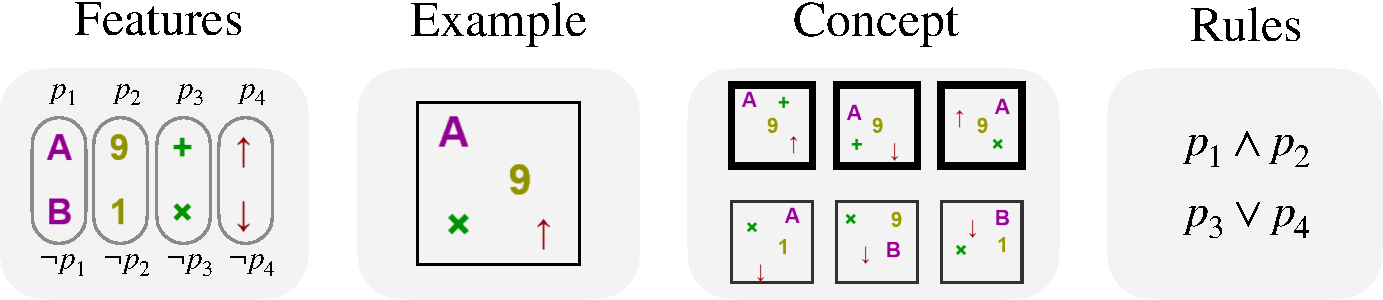
\includegraphics[scale=.6]{papers/images_behavior_research_methods/intro_notation.pdf}
% \end{center}\caption{Illustration of the features $\{p_1,p_2,p_3,p_4\}$, the example $(1,1,0,1)$, and a concept (positive example are marked with bold boundaries and negative examples with thin boundaries). The concept can be explained with the two minimal rules $p_1 \land p_2$ or $p_3 \lor p_4$, depending on which features are used to build the rule (the first two features or the last two features, respectively).}
	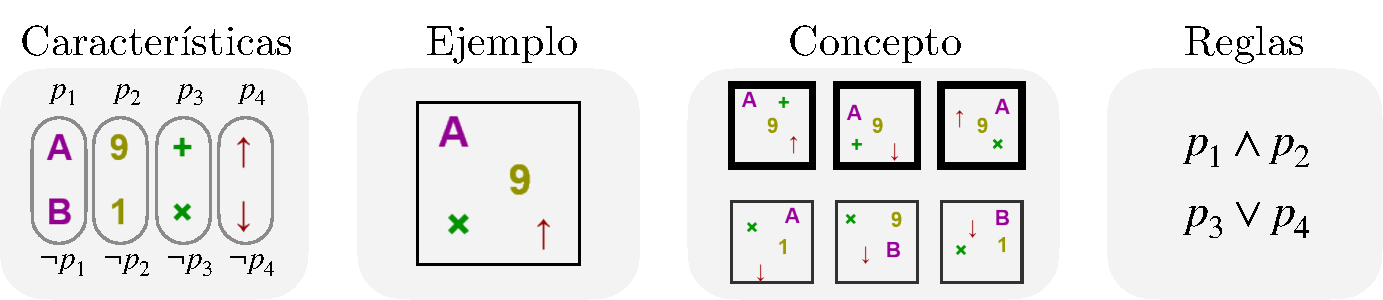
\includegraphics[scale=.6]{papers/images_behavior_research_methods/intro_notation_sp.pdf}
\end{center}\caption{Ilustración de las características $\{p_1,p_2,p_3,p_4\}$, el ejemplo $(1,1,0,1)$, y un concepto (los ejemplos positivos están marcados con marcos gruesos y los ejemplos negativos con marcos delgados). El concepto se puede explicar con las dos reglas mínimas $p_1 \land p_2$ o $ p_3 \lor p_4$, dependiendo de las características que se usen para construir la regla (las dos primeras características o las dos últimas características, respectivamente).}
\label{fig:intro_notation}
\end{figure}



% In propositional concept-learning experiments, participants are presented with a set of \textit{examples}, each conformed of $N$ propositional \textit{features}, which can take positive or negative values. For instance, for $N=4$ one example can be logically represented as the element $(1,1,0,1)$, which takes positive values for the first, second and fourth features and negative for the second one, as illustrated in Figure~\ref{fig:intro_notation}. A \textit{concept} can be intuitively understood as a set of examples, some of them marked as belonging to the concept and the rest marked as not belonging, i.e.\ positive and negative examples. In Figure~\ref{fig:intro_notation} we show an example of an \textit{underdetermined} concept, in the sense that, since the entire universe of examples is not shown (i.e. the $2^4$ possibilities), different determined concepts can be consistent with this smaller set when extending the set of examples to the full universe. 
En los experimentos de aprendizaje de conceptos proposicionales, a los participantes se les presenta un conjunto de \textit{ejemplos}, cada uno conformado por $N$ \textit{features} proposicionales, que pueden tomar valores positivos o negativos. Por ejemplo, para $N=4$ un ejemplo se puede representar lógicamente como el elemento $(1,1,0,1)$, que toma valores positivos para la primera, segunda y cuarta características y negativos para la segunda, como ilustramos en la Figura ~\ref{fig:intro_notation}. Un \textit{concepto} puede entenderse intuitivamente como un conjunto de ejemplos, algunos de ellos marcados como pertenecientes al concepto y el resto marcados como no pertenecientes, es decir, ejemplos positivos y negativos. En la Figura~\ref{fig:intro_notation} mostramos un ejemplo de un concepto \textit{subdeterminado}, en el sentido de que, dado que no se muestra universo completo de ejemplos (es decir, las $2^4$ posibilidades), diferentes conceptos determinados pueden ser coherentes con este conjunto más pequeño al extender el conjunto de ejemplos al universo completo.


% A \textit{rule} consistent with the concept is a logical formula built with the features and the conjunction ($\land$), disjunction ($\lor$), and negation ($\lnot$) operators, which evaluates to true for objects belonging to the concept and false otherwise (e.g.\ $p_1 \land p_2$, where $p_i$ is the $i^{th}$ feature, see Figure~\ref{fig:intro_notation}). The \textit{minimal description length} (\textit{MDL}) of a concept is the length of the shortest rule consistent with the concept~\cite{grunwald2007minimum} (here, the {\em length} of a formula is defined as the number of positive or negative occurrences of propositional symbols plus the number of occurrences of operators $\land$ or $\lor$ contained in it; for example, the length of $p_1 \land \lnot p_3$ is 3, and the length of $(p_1 \land \lnot p_3)\lor p_2$ is 5). Importantly, most studies of subjective difficulty with concept-learning are designed such that a {\em single} minimal rule can be used to describe the concept (e.g.\ $p_1 \land p_2$)~\cite{ashby2005human,feldman2000minimization}, even when the difficulty of finding the features that compose that rule ($p_1$ and $p_2$) is measured with attention-tracking mechanisms (e.g.\~\cite{blair2009extremely,hoffman2010costs}). This limitation is possibly due to the prohibitively large number of rules that can be built with a given set of features, making it difficult to control which rules the participant might use when observing a set of examples. For instance, in order to determine the difficulty that participants have in learning the logical rule $p_1 \lor p_2$, it is crucial to control that no other rule of reasonable complexity can explain the concept (e.g.\ $p_1 \land p_3$). In this work, we use the tools of propositional logic to build an experimental framework that allows us to present examples consistent with two (or more) chosen rules, depending on which features are observed. For instance, the concept shown in Figure~\ref{fig:intro_notation} is consistent with the explanation $p_1 \land p_2$ \textit{and also} with the explanation $p_3 \lor p_4$, depending on which features are observed. In general, the experimenter can choose any pair of rules that use any number of (non-overlapping) features, and our framework guarantees that the presented examples are only consistent with the two minimal rules chosen by the experimenter. Then, by presenting novel examples that are consistent with only one of the previous rules, the experimenter can determine which rule the participants internally used to learn the concept, and thus which features they attended to.
Una \textit{regla} consistente con el concepto es una fórmula lógica construida con las características y los operadores de conjunción ($\land$), disyunción ($\lor$) y negación ($\lnot$), que se evalúa como verdadera para objetos que pertenecen al concepto y falsa en caso contrario (por ejemplo, $p_1 \land p_2$, donde $p_i$ es la $i$-ésima característica, ver Figura~\ref{fig:intro_notation}). La \textit{longitud mínima de descripción} (\textit{MDL} por sus siglas en inglés) de un concepto es la longitud de la regla más corta consistente con el concepto~\cite{grunwald2007minimum} (aquí, la {\em longitud} de una fórmula se define como número de apariciones positivos o negativos de símbolos proposicionales, más el número de apariciones de los operadores $\land$ o $\lor$ contenidos en él; por ejemplo, la longitud de $p_1 \land \lnot p_3 $ es 3, y la longitud de $(p_1 \land \lnot p_3) \lor p_2$ es 5). Es importante destacar que la mayoría de los estudios sobre la dificultad subjetiva en el aprendizaje de conceptos están diseñados de manera que se pueda usar una {\em única} regla mínima para describir el concepto (por ejemplo, $p_1 \land p_2$)~\cite{ashby2005human,feldman2000minimization}, incluso cuando la dificultad de encontrar las características que componen esa regla ($p_1$ y $p_2$) se mide con mecanismos de seguimiento de atención (por ejemplo,~\cite{blair2009extremely, hoffman2010costs}). Esta limitación se debe posiblemente a la cantidad prohibitivamente grande de reglas que se pueden construir con un conjunto de características dado, lo que dificulta el control de las reglas que el participante podría usar al observar un conjunto de ejemplos. Por caso, para determinar la dificultad que tienen los participantes en aprender la regla lógica $p_1 \lor p_2$, es crucial controlar que ninguna otra regla de complejidad razonable pueda explicar el concepto (por ejemplo, $p_1 \land p_3$). En este trabajo, utilizamos las herramientas de la lógica proposicional para construir un marco experimental que nos permita presentar ejemplos consistentes con dos (o más) reglas elegidas, dependiendo de qué características se observen. Por ejemplo, el concepto mostrado en la Figura~\ref{fig:intro_notation} es consistente con la explicación $p_1 \land p_2$ \textit {y también} con la explicación $p_3 \lor p_4$, dependiendo de qué características se observen. En general, el experimentador puede elegir cualquier par de reglas que usen cualquier número de características (no superpuestas), y nuestro marco garantiza que los ejemplos presentados solo son consistentes con las dos reglas mínimas elegidas por el experimentador. Luego, al presentar ejemplos novedosos que sean consistentes con solo una de las reglas anteriores, el experimentador puede determinar qué regla usaron los participantes internamente para aprender el concepto y, por lo tanto, a qué características atendieron.


% Presenting rules $A$ and $B$ (e.g.\ $p_1 \land p_2$ and $p_3 \lor p_4$) using the same set of examples has several experimental advantages over separately presenting a set of examples consistent with rule $A$ and then a set of examples consistent with rule $B$. Some of the advantages are: 
Presentar las reglas $A$ y $B$ (por ejemplo, $p_1\land p_2$ y $p_3 \lor p_4$) utilizando el mismo conjunto de ejemplos tiene varias ventajas experimentales sobre la presentación por separado de un conjunto de ejemplos coherentes con la regla $A$ y luego un conjunto de ejemplos consistentes con la regla $B$. Algunas de las ventajas son:

\begin{enumerate}
\item [(1)] 
% When comparing the relative difficulty of learning $A$ and $B$ in the same participant, presenting the examples separately makes it hard to overcome transfer effects that cause subjective difficulty to depend on the history of concepts learnt previously in the task, and cause different relative difficulties if $A$ is learnt before $B$ compared to $B$ being learnt before $A$ (see for example~\cite{tano2020towards}). The experimenter could compare learning times for $A$ and $B$ across participants, but for reasonably hard rules there are very large idiosyncratic differences in learning difficulties which greatly increases the variance of learning times (see for example~\cite{feldman2000minimization}), and also the experimenter cannot normalize the past history of each participant before the experiment. On the other hand, presenting $A$ and $B$ simultaneously via the same set of examples allows us to directly measure which of the two rules is most easily found by the participant, when the two are presented under exactly the same experimental conditions.
Cuando comparamos la dificultad relativa de aprender $A$ y $B$ en el mismo participante, si presentamos los ejemplos por separado, se complica superar los efectos de transferencia que hacen que la dificultad subjetiva dependa de la historia de conceptos aprendidos previamente en la tarea, y provoquen diferentes dificultades relativas si $A$ se aprende antes de $B$ en comparación a si $B$ se aprende antes de $A$ (ver por ejemplo~\cite{tano2020towards}). El experimentador podría comparar los tiempos de aprendizaje para $A$ y $B$ entre los participantes, pero para reglas razonablemente estrictas, existen diferencias idiosincrásicas muy grandes en las dificultades de aprendizaje que aumentan enormemente la variación de los tiempos de aprendizaje (ver, por ejemplo,~\cite{feldman2000minimization}). Además, el experimentador no puede normalizar la historia pasada de cada participante antes del experimento. Por otro lado, presentar $A$ y $B$ simultáneamente a través del mismo conjunto de ejemplos nos permite medir directamente cuál de las dos reglas encuentra más fácilmente el participante, cuando las dos se presentan exactamente bajo las mismas condiciones experimentales.

\item [(2)] 
% The fact that rule $A$ is learnt more easily than $B$ when presented separately does not necessarily mean that the same happens when presented jointly. This could not hold if there is an interaction between the logical operators being learnt (that compose the rules $A$ and $B$) and the search mechanism used to find the corresponding rules. For instance, the search mechanism that allows humans to find a disjunction rule consistent with the examples could interact with the mechanism that allows to find conjunctions, an interaction that could only be characterized when the conjunction and disjunction are presented at the same time.
El hecho de que la regla $A$ se aprenda más fácilmente que $B$ cuando se presentan por separado no significa necesariamente que suceda lo mismo cuando se presenta en conjunto. Esto no podría ser válido si existiera una interacción entre los operadores lógicos que se están aprendiendo (que componen las reglas $A$ y $B$) y el mecanismo de búsqueda utilizado para encontrar las reglas correspondientes. Por ejemplo, el mecanismo de búsqueda que permite a los humanos encontrar una regla de disyunción consistente con los ejemplos podría interactuar con el mecanismo que permite encontrar conjunciones, interacción que solo podría caracterizarse cuando la conjunción y la disyunción se presentan al mismo tiempo.

\item [(3)] 
% Our framework allows us to test second-order subjective difficulty effects (e.g.\ rule $A$ is learnt faster if presented jointly with rule $B$ than with rule $C$), as well as second-order transfer learning effects (e.g.\  participants learn more rapidly rule $C$ if they have first observed rule $A$ jointly presented with an arbitrary rule $B_1$, compared to $A$ coupled with a different rule $B_2$).
Nuestro marco nos permite probar efectos de dificultad subjetiva de segundo orden (por ejemplo, la regla $A$ se aprende más rápido si se presenta junto con la regla $B$ que si se presenta junto con la regla $C$), así como efectos de aprendizaje de transferencia de segundo orden (por ejemplo, los participantes aprenden más rápidamente la regla $C$ si primero han observado la regla $A$ presentada conjuntamente con una regla arbitraria $B_1$, en comparación con $ $ junto con una regla diferente $B_2$).

\item [(4)] 
% If one is interested in which features are preferentially observed by the participant in a given trial (e.g.\  features $\{p_1,p_2\}$ or $\{p_3,p_4\}$), one could simply choose the same logical structure for $A$ and $B$ (e.g.\ making $A$ and $B$ equal to $p_1 \land p_2$ and $p_3 \land p_4$) and test whether $A$ or $B$ is learnt by the participant. Then, any preference for learning $A$ over $B$ could only be due to a preference over the features themselves ($\{p_1,p_2\}$), and not for the logical description of the concept using those features (this is, $\boldsymbol{\cdot} \land \boldsymbol{\cdot}$).
Si uno está interesado en qué características observa preferentemente el participante en una prueba determinada (por ejemplo, las características $\{p_1, p_2 \}$ o $\{p_3, p_4 \} $), simplemente se podría elegir la misma estructura lógica por $A$ y $B$ (por ejemplo, haciendo que $A$ y $B$ sean iguales a $p_1 \land p_2$ y $p_3 \land p_4 $) y comprobar si el participante aprende $A$ o $B$ . Entonces, cualquier preferencia por aprender $A$ sobre $B$ solo podría deberse a una preferencia sobre las características en sí mismas ($\{p_1, p_2 \} $), y no por la descripción lógica del concepto que usa esas características (esto es, $\boldsymbol{\cdot} \land \boldsymbol{\cdot}$).
\end{enumerate}



% We illustrate these advantages in an experiment in which participants are presented with a sequence of 6 trials, observing in each trial a set of examples consistent with two alternative rules. We illustrate advantage (1) and (2) discussed above by presenting a conjunction together with a disjunction; and a simple rule together with a complex rule. Then, we show that after observing in several trials that a subset of features is useful to find concise rules, we induce  in the participants a bias to preferentially describe concepts using those features; this bias was tested exploiting  advantage (4).
Ilustramos estas ventajas en un experimento en el que a los participantes se les presenta una secuencia de 6 pruebas, observando en cada prueba un conjunto de ejemplos consistentes con dos reglas alternativas. Ilustramos la ventaja (1) y (2) discutida anteriormente presentando una conjunción junto con una disyunción; y una regla simple junto con una regla compleja. Luego, mostramos que después de observar en varias pruebas que un subconjunto de características es útil para encontrar reglas concisas, inducimos en los participantes un sesgo para describir conceptos usando preferentemente esas características; este sesgo se probó aprovechando la ventaja (4).





%!TEX root = Main.tex

\section{Experimento}\label{Section:Experiment}

\subsection{Participantes} \label{Participants}

% The experiment was conducted as a Human Intelligence Task (HIT) in Amazon's Mechanical Turk~\cite{crump2013evaluating, buhrmester2011amazon, stewart2015average}. There were 100 participants,  self-selected workers that saw, accepted, and finished the published HIT. We required workers to have a HIT approval rate of $95\%$ or more. Workers were informed that the payment for completing the experiment was going to be of {1.5} US dollars, and that 1 out of 20 participants would be randomly assigned a bonus of 10 dollars, regardless of their performance in the experiment's tasks as long as they finished the experiment (but note that trials did not end until they correctly learned each concept).
El experimento se llevó a cabo como una tarea de Human Intelligence Task (HIT) en Mechanical Turk~\cite{crump2013evaluating, buhrmester2011amazon, stewart2015average} de Amazon. Hubo 100 participantes, trabajadores autoseleccionados que vieron, aceptaron y terminaron el HIT publicado. Requerimos que los trabajadores tuvieran una tasa de aprobación HIT de $95 \%$ o más. Se informó a los trabajadores que el pago por completar el experimento sería de {1,5} dólares estadounidenses,
y que a 1 de cada 20 participantes se le asignaría aleatoriamente una bonificación de 10 dólares, independientemente de su desempeño en las tareas del experimento, siempre que terminaran el experimento (pero tener en cuenta que las pruebas no terminaron hasta que aprendieron correctamente cada concepto).

% For exclusion criteria, see the appendix~\S\ref{Sec:ExclusionCriteria}.
Para conocer los criterios de exclusión, consultar el apéndice~\S\ref{Sec:ExclusionCriteria}.


\subsection{Configuración del experimento}\label{Subsec:ExperimentFlow}
% The main idea of our experimental framework is schematized in Figure~\ref{fig:twoconcepts}. The participants observe an \textit{underdetermined} concept. This concept is presented to the participants as a set of elements that belong to it (positive examples), and a set of elements that do not (negative examples). In  Figure~\ref{fig:twoconcepts}, the elements marked as positive examples are the ones in the intersection of the two concepts and the negative examples are the ones outside of both concepts. Importantly, the listing is incomplete, in the sense that not all elements of the universe are shown. The critical insight is that, when extending the set of examples to the full universe, there is more than one possible concept that is consistent with the observed examples.  For example, in Figure~\ref{fig:twoconcepts},  the presented examples are consistent with the minimal rule of $C_1$ (i.e.\ $\varphi_1=p_1\lor p_2$) \textit{and also} with the minimal rule of $C_2$ (i.e.\ $\varphi_2=p_3\land p_4$). As we explain in the rest of this section, choosing $C_1$ and $C_2$ appropriately can be exploited to control the minimal rules that are consistent with the examples that participants observe.
La idea principal de nuestro marco experimental se esquematiza en la Figura~\ref{fig:twoconcepts}. Los participantes observan un concepto \textit{indeterminado}. Este concepto se presenta a los participantes como un conjunto de elementos que le pertenecen (ejemplos positivos), y un conjunto de elementos que no (ejemplos negativos). En la Figura~\ref{fig:twoconcepts}, los elementos marcados como ejemplos positivos son los que están en la intersección de los dos conceptos y los ejemplos negativos son los que están fuera de ambos conceptos. Es importante destacar que la lista es incompleta, en el sentido de que no se muestran todos los elementos del universo. La idea fundamental es que, al extender el conjunto de ejemplos al universo completo, hay más de un concepto posible que es consistente con los ejemplos observados. Por ejemplo, en la Figura~\ref{fig:twoconcepts}, los ejemplos presentados son consistentes con la regla mínima de $C_1$ (es decir, $\varphi_1 = p_1 \lor p_2$) \textit {y también} con la regla mínima de $C_2$ (es decir, $\varphi_2 = p_3 \land p_4$). Como explicamos en el resto de esta sección, la elección adecuada de $C_1$ y $C_2$ puede aprovecharse para controlar las reglas mínimas que son consistentes con los ejemplos que observan los participantes.


\begin{figure}
\begin{center}
	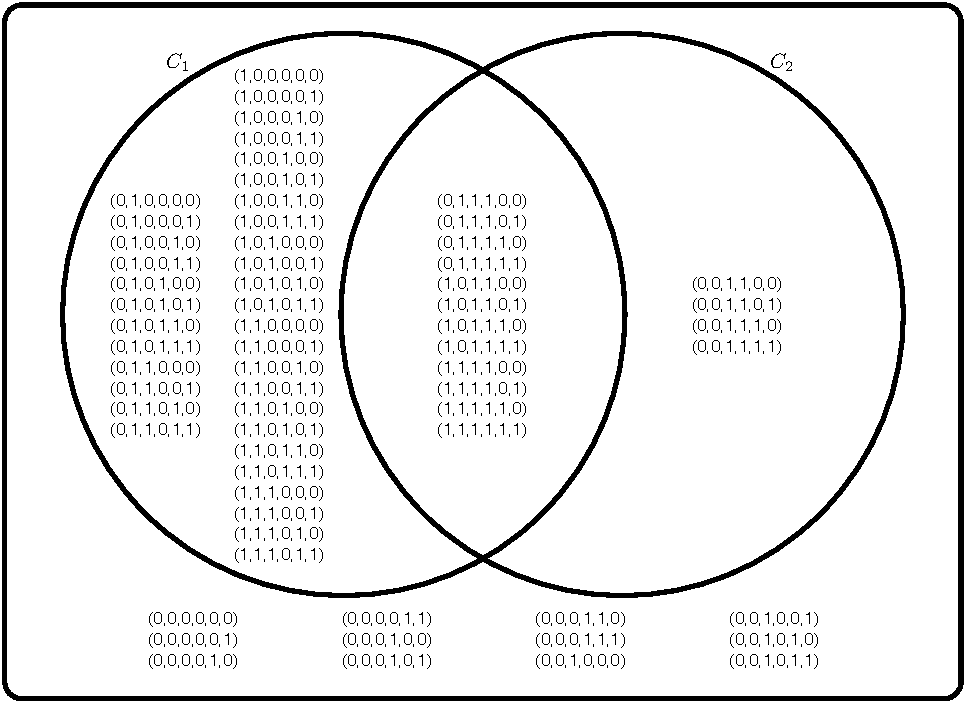
\includegraphics[scale=.65]{papers/images_behavior_research_methods/twoconcepts3.pdf}
\end{center}\caption{
%An example of a pair of concepts $C_1$ and $C_2$ with 6 features. Concept $C_1$ can be described by $\varphi_1=p_1 \lor p_2$, and $C_2$ by $\varphi_2=p_3\land p_4$. This is just a schematic illustration of where each element (tuple) is placed with respect to concepts. These concepts correspond to the ones used in Trial 1 of the actual experiment. However, elements in the actual experiment are not represented in this way (i.e.\ as tuples of zeroes and ones).
Un ejemplo de un par de conceptos $C_1$ y $C_2$ con 6 características. El concepto $C_1$ puede ser descrito por $\varphi_1 = p_1 \lor p_2 $, y $C_2$ por $\varphi_2 = p_3 \land p_4$. Esta es solo una ilustración esquemática de dónde se coloca cada elemento (tupla) con respecto a los conceptos. Estos conceptos corresponden a los utilizados en la Prueba 1 del experimento real. Sin embargo, los elementos del experimento real no se representan de esta manera (es decir, como tuplas de ceros y unos).
}
\label{fig:twoconcepts}
\end{figure} 

% The actual experiment that we implemented consists of a sequence of 6 trials constructed in this manner. We now expand the 3 stages that compose each $i$-th trial of the experiment. For a better understanding, see Figure~\ref{fig:trials}, which consists of a schematic view of one trial. Note that this figure is merely illustrative and does not aim to describe the details of a trial, but rather the sequence of phases and the logical flow within a trial. In particular, note that the number of elements {\sf A}'s, {\sf B}'s, {\sf C}'s and {\sf D}'s in the figure are not meaningful, as they vary from trial to trial along the experiment. The actual concepts used in each trial, as well as the number of positive and negative examples is listed in Table~\ref{trial_table} (groups X,Y are only relevant for Hypothesis III, so they can be ignored for now), and more details of the actual implementation can be found in \S\ref{sub:experimentdetails} and \S\ref{FullExperimentDescription}.
El experimento real que implementamos consiste en una secuencia de 6 pruebas, cada una de las cuales está construida de esta manera. Ahora expandimos las 3 etapas que componen la $i$-ésima prueba del experimento. Para una mejor comprensión, consultar la Figura~\ref{fig:trials}, que consiste en una vista esquemática de una prueba. Tenga en cuenta que esta figura es meramente ilustrativa y no pretende describir los detalles de una prueba, sino más bien la secuencia de fases y el flujo lógico dentro de una prueba. En particular, tener en cuenta que el número de elementos {\sf A}, {\sf B}, {\sf C} y {\sf D} en la figura no son significativos, ya que varían de prueba en prueba a lo largo del experimento. Los conceptos reales utilizados en cada ensayo, así como el número de ejemplos positivos y negativos se enumeran en la Tabla~\ref{trial_table} (los grupos X, Y solo son relevantes para la Hipótesis \ref{Hip:FeatureBiasTimeAdvantage}, por lo que pueden ignorarse por ahora), y se pueden encontrar más detalles de la implementación real en \S\ref{sub:experimentdetails} y \S\ref{FullExperimentDescription}.  
 \begin{figure}[t]
\begin{center}
	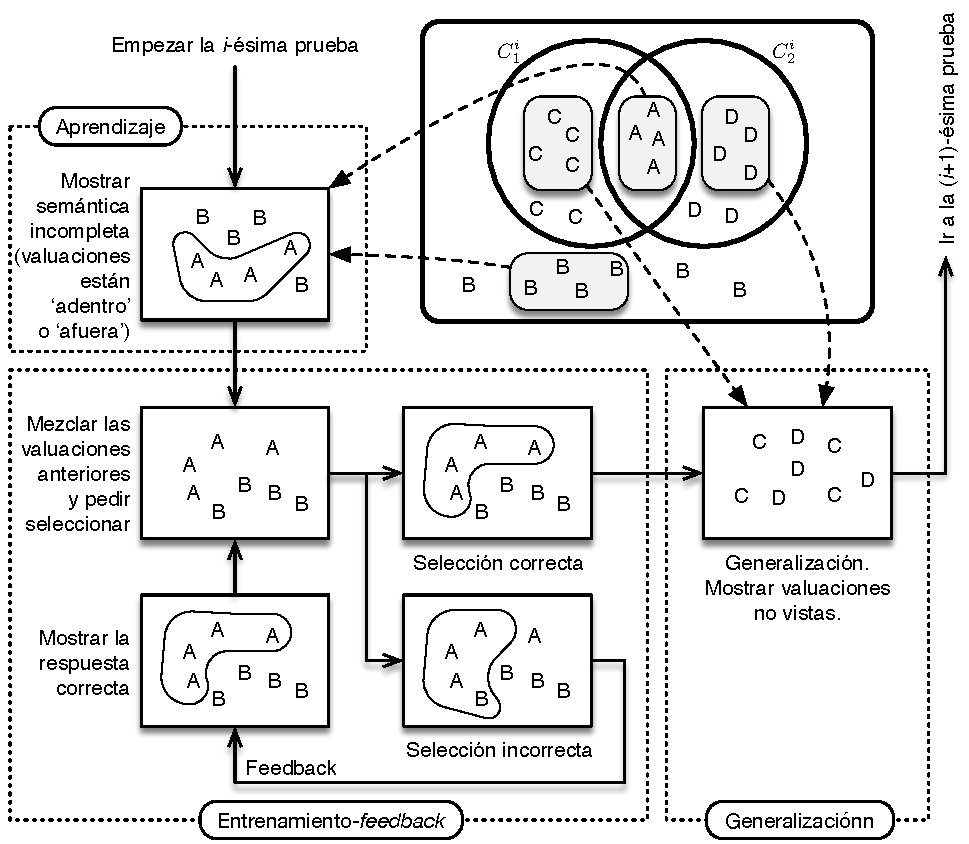
\includegraphics[scale=.7]{papers/images_behavior_research_methods/experimentscheme2_sp.pdf}
\end{center}\caption{
% The scheme of our experimental framework for studying concept learning in the presence of multiple explanations. We illustrate the three phases that constitute each trial: learning phase, training-feedback phase and generalization phase. Elements are represented with letters {\sf A}, {\sf B}, {\sf C} and {\sf D} (for example, the four letters {\sf A} in the intersection represent four different elements in the intersection). The depicted number of such letters {\sf A}, {\sf B}, {\sf C} or {\sf D} is irrelevant (for example, there would be 12 {\sf A}s and 4 {\sf D}s for concepts of Figure~\ref{fig:twoconcepts}).
El esquema de nuestro marco experimental para estudiar el aprendizaje de conceptos en presencia de múltiples explicaciones. Ilustramos las tres fases que constituyen cada ensayo: fase de aprendizaje, fase de formación-{\em feedback} y fase de generalización. Los elementos se representan con las letras {\sf A}, {\sf B}, {\sf C} y {\sf D} (por ejemplo, las cuatro letras {\sf A} en la intersección representan cuatro elementos diferentes en la intersección). El número representado de tales letras {\sf A}, {\sf B}, {\sf C} o {\sf D} es irrelevante (por ejemplo, habría 12 {\sf A}s y 4 {\sf D}s para los conceptos de la Figura~\ref{fig:twoconcepts}).
  }
\label{fig:trials}
\end{figure}

\begin{enumerate}
    % \item \label{item:LearningStage}{\bf Learning stage.} The participant is exposed to a set of `in' elements corresponding to $C^i_1\cap C^i_2$ (marked as `{\sf A}' in Figure~\ref{fig:trials}), and a set of `out' elements corresponding to the {\em complement} of $C^i_1\cup C^i_2$ (marked as `{\sf B}' in Figure~\ref{fig:trials}). 
    \item \label{item:LearningStage}{\bf Etapa de aprendizaje.} El participante se expone a un conjunto de elementos `adentro' correspondientes a $ C^i_1\cap C^i_2$ (marcados como `{\ sf A}' en la Figura~\ref{fig:trials}), y un conjunto de Elementos `afuera' correspondientes al {\em complemento} de $C^i_1\cup C^i_2$ (marcados como` {\sf B}' en la Figura~ ref{fig:trials}).

    
    % We call these shown elements `positive examples' and `negative examples', respectively. Note that this information is incomplete, in the sense that not all possible examples are shown to the participant (as the only examples that are shown from $C^i_1\cup C^i_2$ are those in $C^i_1\cap C^i_2$). In the illustrative example of Figure~\ref{fig:twoconcepts} (corresponding to concepts of Trial 1 of the actual experiment), 24 elements would be shown: the 12 positive examples in the intersection of $C_1$ and $C_2$, and the 12 negative examples outside of both $C_1$ and $C_2$. The participant is asked to learn the concept represented by positive examples.
	A estos elementos mostrados los llamamos `ejemplos positivos' y `ejemplos negativos', respectivamente. Hay que tener en cuenta que esta información es incompleta, en el sentido de que no todos los ejemplos posibles se muestran al participante (ya que los únicos ejemplos que se muestran de $C^i_1 \cup C^i_2$ son los de $C^i_1 \cap C^i_2$). En el ejemplo ilustrativo de la Figura~\ref{fig:twoconcepts} (correspondiente a los conceptos de la Prueba 1 del experimento real), se mostrarían 24 elementos: los 12 ejemplos positivos en la intersección de $C_1$ y $C_2$, y los 12 ejemplos negativos fuera de $C_1$ y fuera de $C_2$. Se pide al participante que aprenda el concepto representado por ejemplos positivos.

 	% As we prove formally in Appendix \ref{Sec:MainTheoremConcept}, the experimental design guarantees that there are only two propositional rules ($\varphi_1$ and $\varphi_2$ in Figure~\ref{fig:twoconcepts}), minimal over their respective sets of features, such that: \textit{(1)} they are \textit{consistent} explanations for shown examples (this is, they satisfy positive examples but do not satisfy negative examples), \textit{(2)} they use different features from each other (e.g.\ $\{p_1, p_2\}$ in $\varphi_1$ and $\{p_3,p_4\}$ in $\varphi_2$)  and, importantly, \textit{(3)} \textit{any} rule consistent with the examples must use a superset of the set of features of at least one of these minimal rules. For instance, in Figure~\ref{fig:twoconcepts} any rule that only uses $\{p_2, p_3\}$ cannot explain the examples, since $(1,{\bf 0},{\bf 1},1,1,1)$ is a positive example but  $(0,{\bf 0},{\bf 1},0,1,1)$  is a negative example. Any rule that can consistently explain the examples must mention a superset of $\{p_1, p_2\}$ (e.g.\  $\{p_1, p_2, p_3\}$) or a superset of $\{p_3, p_4\}$. The proof of this condition is shown in Theorem \ref{theorem:TeoremaPrincipal}, but we also sketch it  here. Observe that in Figure~\ref{fig:twoconcepts} the negative example  $(0,{\bf 0},{\bf 1},0,1,1)$  was constructed from the positive example  $(1,{\bf 0},{\bf 1},1,1,1)$ by flipping the values of $p_1$ and $p_4$, and doing so results in an element that is inconsistent with both $\varphi_1$ and $\varphi_2$. When an alternative explanation leaves unused some features $p,q$ that appear in $\varphi_1$ and $\varphi_2$ respectively, there must be some element that satisfies both rules $\varphi_1,\varphi_2$, but none of them is satisfied when the values of $p$ and $q$ are flipped. Since the truth value of the alternative rule is maintained when features that do not appear in it change, and since we are showing as positive examples all elements that satisfy both rules $\varphi_1,\varphi_2$ and as negative examples all those that satisfy none of them, such alternative explanation must be inconsistent with the shown data.
	Como demostramos formalmente en el Apéndice \ref{Sec:MainTheoremConcept}, el diseño experimental garantiza que solo hay dos reglas proposicionales ($\varphi_1$ y $\varphi_2$ en la Figura~\ref{fig:twoconcepts}), mínimas sobre sus respectivos conjuntos de características, tales que: \textit{(1)} son explicaciones \textit{consistentes} con los ejemplos mostrados (esto es, satisfacen los ejemplos positivos pero no satisfacen los ejemplos negativos), \textit{(2)} usan características diferentes entre sí (por ejemplo, $\{p_1, p_2 \}$ en $\varphi_1$ y $\{p_3, p_4 \}$ en $\varphi_2 $) y, lo que es más importante, \textit {(3)} \textit{cualquier} regla consistente con los ejemplos debe usar un superconjunto del conjunto de características de al menos una de estas reglas mínimas. Por ejemplo, en la Figura~\ref{fig:twoconcepts} cualquier regla que solo use $\{p_2, p_3 \}$ no puede explicar los ejemplos, ya que $(1, {\bf 0}, {\bf 1}, 1 , 1,1)$ es un ejemplo positivo, pero $(0, {\bf 0}, {\bf 1}, 0,1,1)$ es un ejemplo negativo. Cualquier regla que pueda explicar consistentemente los ejemplos debe mencionar un superconjunto de $\{p_1, p_2 \}$ (por ejemplo, $\{p_1, p_2, p_3 \}$) o un superconjunto de $\{p_3, p_4 \}$. La prueba de esta condición se muestra en el Teorema \ref{theorem:TeoremaPrincipal}, pero también lo esbozamos aquí. Observar que en la Figura~\ref{fig:twoconcepts} el ejemplo negativo $(0, {\bf 0}, {\bf 1}, 0,1,1)$ se construyó a partir del ejemplo positivo $(1, {\bf 0}, {\bf 1}, 1,1,1)$ invirtiendo los valores de $p_1$ y $p_4$, y hacerlo da como resultado un elemento que es inconsistente tanto con $\varphi_1$ como con $\varphi_2$. Cuando una explicación alternativa deja sin usar algunas características $p,q$ que aparecen en $\varphi_1$ y $\varphi_2$ respectivamente, debe haber algún elemento que satisfaga ambas reglas $\varphi_1, \varphi_2$, pero ninguna de ellas es satisfecha cuando se invierten los valores de $p$ y $q$. Dado que el valor de verdad de la regla alternativa se mantiene cuando cambian características que no aparecen en ella, y dado que estamos mostrando como ejemplos positivos todos los elementos que satisfacen ambas reglas $\varphi_1, \varphi_2$ y como ejemplos negativos todos aquellos que no satisfacen ninguno de ellos, dicha explicación alternativa debe ser inconsistente con los datos mostrados.

	% These three conditions guarantee that the experimental procedure illustrated in Figure~\ref{fig:twoconcepts} is a logically sound method to present a concept consistent with two minimal rules chosen by the experimenter ($\varphi_1$ and $\varphi_2$), depending on which features the participant use to build the rule.
	Estas tres condiciones garantizan que el procedimiento experimental ilustrado en la Figura~\ref{fig:twoconcepts} es un método lógicamente sólido para presentar un concepto consistente con dos reglas mínimas elegidas por el experimentador ($\varphi_1$ y $\varphi_2$), dependiendo sobre qué características se basa el participante para construir la regla.    

    % \item {\bf Training-feedback stage.} The {\em same} examples of the learning stage are shown to the participant, but this time without indicating whether they are negative or positive and in a shuffled order. The participant is asked to tag each element as `in' or `out', in the same way they were tagged in the previous step. If all elements are classified correctly, the participant proceeds to the next stage. Otherwise, the participant is informed about the mistakes in their tagging, and after that the training-feedback stage starts again.
    \item {\bf Etapa de entrenamiento-{\em feedback}}. Los {\em mismos} ejemplos de la etapa de aprendizaje se muestran al participante, pero esta vez sin indicar si son negativos o positivos y en orden aleatorio. Se le pide al participante que etiquete cada elemento como `adentro' o `auera', de la misma manera que se etiquetaron en el paso anterior. Si todos los elementos están clasificados correctamente, el participante pasa a la siguiente etapa. De lo contrario, se informa al participante sobre los errores en su etiquetado, y después de eso, la etapa de capacitación-{\em feedback} comienza nuevamente.


    % \item {\bf Generalization stage.} {\em Previously unseen} elements are shown to the participant\footnote{With the exception of Trial 6, where one element is reshown in order to better test Hypothesis~\ref{Hip:FeatureBiasStickiness}. See \S\ref{sec:hypothesis}.}. These elements are taken from $C^i_1\setminus C^i_2$ and from $C^i_2\setminus C^i_1$ (here, `$\setminus$' denotes set difference). These elements are respectively marked as `{\sf C}' and `{\sf D}' in the scheme of Figure~\ref{fig:trials}. The participant is asked to identify those elements that correspond to the concept learnt in the learning stage. After they do so,  the next trial starts. If the participant selects those in $C^i_1\setminus C^i_2$, the concept learnt in the Learning stage was $C^i_1$, and if the participant selects those in $C^i_2\setminus C^i_1$, the concept they learned was $C^i_2$.
    % Continuing with the example from Figure~\ref{fig:twoconcepts}, this process would allow us to determine if the participant was thinking in a rule with the features $\{p_1, p_2\}$ (namely, $\varphi_1$) or $\{p_3, p_4\}$ (namely, $\varphi_2$) to explain the concept. Of course, in practice the participant can select other elements, with no clear rationale.
	\item {\bf Etapa de generalización.} {\em Los elementos no vistos anteriormente} se muestran al participante\footnote{Con la excepción de la Prueba 6, donde un elemento se vuelve a mostrar para testear mejor la Hipótesis~\ref{Hip:FeatureBiasStickiness}. Ver \S\ref{sec:hypothesis}.}. Estos elementos se toman de $C^i_1 \setminus C^i_2$ y de $C^i_2 \setminus C^i_1$ (aquí, `$\setminus$ ' denota la diferencia de conjuntos). Estos elementos están marcados respectivamente como `{\sf C}' y `{\sf D}' en el esquema de la Figura~\ref{fig:trials}. Se pide al participante que identifique aquellos elementos que corresponden al concepto aprendido en la etapa de aprendizaje. Después de hacerlo, comienza la siguiente prueba. Si el participante selecciona los de $C^i_1 \setminus C^i_2$, el concepto aprendido en la etapa de Aprendizaje fue $C^i_1$, y si el participante selecciona los de $C i_2 \setminus C^i_1$, el concepto que aprendieron fue $C^i_2$.
    Continuando con el ejemplo de la Figura~\ref{fig:twoconcepts}, este proceso nos permitiría determinar si el participante estaba pensando en una regla con las características $\{p_1, p_2 \}$ (es decir, $\ varphi_1$) o $\{p_3, p_4 \}$ (es decir, $\varphi_2$) para explicar el concepto. Por supuesto, en la práctica, el participante puede seleccionar otros elementos, sin una justificación clara.

    % Once the participant chooses the elements, they are asked to write an explanation of what constitutes the concept; this answer is not part of the data analysis, except that it allows us to exclude participants that are using methods outside the scope of the experiment (such as taking pictures). Additionally, the written answers serve as an extra sanity check of whether the participants are actually thinking in a way consistent with the framework of propositional logic (see \S\ref{Sec:ExclusionCriteria} for observations on the written explanations obtained in the experiment).
	Una vez que el participante elige los elementos, se le pide que escriba una explicación de lo que constituye el concepto; esta respuesta no es parte del análisis de datos, excepto que nos permite excluir a los participantes que están usando métodos fuera del alcance del experimento (como tomar fotografías). Además, las respuestas escritas sirven como una {\em sanity check} adicional de si los participantes realmente están pensando de una manera consistente con el marco de la lógica proposicional (ver \S\ref{Sec:ExclusionCriteria} para las observaciones sobre las explicaciones escritas obtenidas en el experimento) .
\end{enumerate}

%More details of the experiment and its structure can be found in Section~\ref{Sec:AdditionalMethodology}, particularly in \S\ref{sub:experimentdetails} and \S\ref{FullExperimentDescription}. 
Se pueden encontrar más detalles del experimento y su estructura en la Sección~\ref{Sec:AdditionalMethodology}, particularmente en \S\ref{sub:experimentdetails} y \S\ref{FullExperimentDescription}. 

% \subsection{Experiment trials}\label{sec:hypothesis}
%     The set of trials chosen in the experiment (Table~\ref{trial_table}) aims to reveal the biases that cause participants to choose one set of features over another in this framework where both sets of features have their own minimal rules consistent with the observed positive and negative examples. For instance, in Figure~\ref{fig:twoconcepts}, what causes participants to choose $\{p_1, p_2\}$ versus $\{p_3, p_4\}$ to explain the concept? Our hypothesis is that a key inductive bias is simply the frequency with which a subset of features was used previously to explain past concepts. We name this bias as \textit{feature stickiness}.
\subsection{Ensayos experimentales}\label{sec:hypothesis}
     El conjunto de pruebas elegidas en el experimento (Tabla~\ref{trial_table}) tiene como objetivo revelar los sesgos que hacen que los participantes elijan un conjunto de características sobre otro en este marco donde ambos conjuntos de características tienen sus propias reglas mínimas consistentes con los ejemplos observados positivos y negativos. Por ejemplo, en la Figura~\ref{fig:twoconcepts}, ¿qué hace que los participantes elijan $\{p_1, p_2 \}$ versus $\{p_3, p_4 \}$ para explicar el concepto? Nuestra hipótesis es que un sesgo inductivo clave es simplemente la frecuencia con la que se utilizó previamente un subconjunto de características para explicar conceptos pasados. Denominamos este sesgo como \textit{característica adherente}.

\renewcommand{\arraystretch}{1.4}
\newcommand{\marcaEnTabla}{{\bullet}}%\checkmark



\begin{table}[h]
\begin{center}
\small

  \begin{tabularx}{\linewidth}{
  |>{\centering\hsize=.5\hsize}X
  |>{\centering\hsize=.7\hsize}X
  |>{\centering\hsize=.75\hsize}X
  |>{\centering\hsize=.75\hsize}X
  |>{\centering\hsize=.7\hsize}X
  |>{\centering\hsize=.3\hsize}X
  |>{\centering\hsize=.3\hsize}X
  |>{\centering\hsize=.3\hsize}X
  |>{\centering\hsize=.3\hsize}X
  |>{\centering\arraybackslash\hsize=.7\hsize}X
  |}
    \cline{1-10}
    \multirow{2}*{\textbf{\footnotesize Prueba}}&
    \multirow{2}*{\textbf{\footnotesize Grupo}}&
    \multirow{2}*{$\mathbf{\varphi^i_1}$}&
    \multirow{2}*{$\mathbf{\varphi^i_2}$}&
    \multirow{2}{4\baselineskip}{\textbf{\footnotesize \ \ Caract.\\ mostradas}}&
    \multicolumn{4}{c|}{\footnotesize\bf\ Hipótesis testeadas}&
    \multirow{2}{3\baselineskip}{\centering\tiny{\textbf{Ejemplos mostrados\\\#Positivos \\ (\#Negativos)}}}\\
    \cline{6-9}
    &&&&&\ref{Hip:AndOverOr}&\ref{Hip:FeatureBiasStickiness}&\ref{Hip:FeatureBiasTimeAdvantage}&\ref{Hip:StickinessFeatureOperator}&\\ 
    \cline{1-10}
    $i = 1$ &  X, Y & $\varA \lor \varB$ 	& $\varC \land \varD $  & \multirow{5}*{$p_1$ to $p_6$} &$\marcaEnTabla$ & && $\marcaEnTabla$ & 12 (12) \\ \cline{1-4} \cline{6-10}
    $i = 2$&  X, Y & $\lnot \varA \land \varB$ 					& $\varC \lor \lnot \varD$ 	 &   & & &&$\marcaEnTabla$& 12 (12) \\    \cline{1-4} \cline{6-10}
    \multirow{2}*{$i = 3$} & X & $\varA \land \varB$ 	& \mdl 15   &     \multirow{2}*{} & \multirow{2}*{} &&\multirow{2}*{$\marcaEnTabla$} &&\multirow{2}*{10 (18)}\\\cline{2-4} 
     & Y & $\varE \land \varF$ 	& \mdl 15  &   &&&&&\\    \cline{1-4} \cline{6-10}
    $i = 4$&  X, Y & $ \lnot \varE \land \varF$ 					&  \mdl 15  &  &&&$\marcaEnTabla$&&10 (18)\\    \cline{1-10}
    $i = 5$&  X, Y & $\varG \land \varH$					& \mdl 15  &  \multirow{2}*{$p_3$ to $p_8$}&&$\marcaEnTabla$&&&10 (18)\\    \cline{1-4} \cline{6-10}
    $i = 6$&  X, Y & $\lnot \varG \land \lnot \varH$					& $\varC \land \varD$ &  &&$\marcaEnTabla$&&&4 (36)\\    \cline{1-10}
    \end{tabularx}

\footnotetext{In the case of $i=3$ and group A, the MDL15 rule was $((\varC \lor (\varD \lor \varE))\land(\lnot\varC \lor((\varD \lor\lnot\varE)\land(\varE \lor \lnot\varD))))$} %Uso \footnotetext porque \footnote no funciona desde la tabla
\caption{
% The trials of the experiment. Here $\varphi^i_1$ and $\varphi^i_2$ represent the two competing concepts $C^i_1$ and $C^i_2$ at the $i$-th trial (we denote each concept by the shortest propositional rule whose semantics describes the concept). By ``MDL15'' we denote a concept whose shortest rule is of length 15 (and made of three propositional symbols other than the competing rule in the corresponding trial, see \S\ref{Resultados:MDLbias} for details). In all trials the full universe size is $2
% ^6=64$, corresponding to all possible elements over 6 propositional features. We indicate how participants were divided into groups X and Y, which was used only for Hypothesis \ref{Hip:FeatureBiasTimeAdvantage}. We also indicate which features were shown in the examples, which hypothesis where tested, and the number of positive and negative examples shown in learning and training phases for each trial.
Las pruebas del experimento. Aquí $\varphi^i_1$ y $\varphi^i_2$ representan los dos conceptos en competencia $C^i_1$ y $C^i_2$ en la $i$-ésima prueba (denotamos cada concepto por la regla proposicional más corta cuya semántica describe el concepto). Por ``MDL15'' denotamos un concepto cuya regla más corta es de longitud 15 (y está compuesta por tres símbolos proposicionales distintos de la regla en competencia en el ensayo correspondiente, ver \S\ref{Resultados:MDLbias} para más detalles). En todas las pruebas, el tamaño total del universo es de $2^6=64$, correspondiente a todos los elementos posibles sobre 6 características proposicionales. Indicamos cómo se dividió a los participantes en los grupos X e Y, que se usó solo para la Hipótesis \ref{Hip:FeatureBiasTimeAdvantage}. También indicamos qué características se muestran en los ejemplos, qué hipótesis se testearon y el número de ejemplos positivos y negativos que se muestran en las fases de aprendizaje y entrenamiento para cada ensayo.}
\label{trial_table}
\end{center}
\end{table}



% We now present the main hypotheses of this work, and their relation with the various experimental trials. 
A continuación presentamos las principales hipótesis de este trabajo y su relación con las distintas pruebas experimentales.

\theoremstyle{definition}
\newtheorem{hyp}{Hipótesis}
\renewcommand\thehyp{\Roman{hyp}}
 

\begin{hyp}\label{Hip:AndOverOr} 
% In Trial 1 we explore whether the same factors that determine rule-learning difficulty when learned in isolation also determine which features participants use when explaining a set of examples consistent with two minimal rules. Particularly, it is well known that concepts involving logical conjunctions are learned faster than concepts involving logical disjunctions~\cite{bourne1970knowing}.
En la Prueba 1, exploramos si los mismos factores que determinan la dificultad en el aprendizaje de las reglas cuando se aprenden de forma aislada también determinan qué características usan los participantes al explicar un conjunto de ejemplos consistentes con dos reglas mínimas. En particular, es bien sabido que los conceptos que involucran conjunciones lógicas se aprenden más rápido que los conceptos que involucran disyunciones lógicas~\cite{bourne1970knowing}.

% In Trial 1, the minimal consistent rule is a disjunction if the observed features are $\{p_1, p_2\}$, and a conjunction if the observed features are $\{p_3, p_4\}$. Importantly, unlike in other concept-learning experiments, both the two-feature disjunction and conjunction are consistent with the observed set of examples. We hypothesize that the learning bias that causes the conjunction to be learnt more easily than the disjunction will also carry over to this framework were both explanations are possible (using different features). As explained before, we use the generalization stage of Trial 1 to determine if participants understood the concept using $\{p_1, p_2\}$ (corresponding to a disjunction) or using $\{p_3, p_4\}$ (corresponding to a conjunction).
En la Prueba 1, la regla mínima consistente es una disyunción si las características observadas son $\{p_1, p_2 \}$, y una conjunción si las características observadas son $\{p_3, p_4 \}$. Es importante destacar que, a diferencia de otros experimentos de aprendizaje de conceptos, tanto la disyunción como la conjunción de dos características son consistentes con el conjunto de ejemplos observado. Presumimos que el sesgo de aprendizaje que hace que la conjunción se aprenda más fácilmente que la disyunción también se trasladará a este marco si ambas explicaciones son posibles (utilizando características diferentes). Como se explicó antes, usamos la etapa de generalización de la Prueba 1 para determinar si los participantes entendieron el concepto usando $\{p_1, p_2 \}$ (correspondiente a una disyunción) o usando $\{p_3, p_4 \} $ (correspondiente a una conjunción).

% This hypothesis was preregistered as:
Esta hipótesis fue pre-registrada como:
\begin{quote}
% In a scenario of two possible explanations for a concept, one of which can be modeled by the logical \AND between two features and other which can be modeled by the \OR between two other features, most people will find the \AND explanation over the \OR explanation.% (Trial 1).     
En un escenario de dos posibles explicaciones para un concepto, una de las cuales puede ser modelada por el \AND lógico entre dos características y otra que puede ser modelada por el \OR lógico entre otras dos características, la mayoría de la gente encontrará la explicación de \AND sobre la explicación de \OR.
\end{quote}
\end{hyp}

\begin{hyp}\label{Hip:FeatureBiasStickiness}
% The \textit{feature stickiness} bias is tested in Trials 5 and 6 of the experiment. After participants have gained sufficient experience with the task, in Trial 5 participants encounter a set of examples consistent with two minimal explanations, a very simple one that uses features $\{p_7, p_8\}$ and a very complex one that uses $\{p_4,p_5,p_6\}$. This leads participants to explain the concept using $\{p_7, p_8\}$, or otherwise they would have to discover an excessively complex explanation. Therefore, we hypothesize that in this case most participants would select the features $\{p_7, p_8\}$\footnote{Note that the features $\{p_5,p_6\}$ that were used in Trial 4 also appear in the MDL15 formula of Trial 5. However, we hypothesized that the extreme complexity of the MDL15 explanation overwheights the possible feature stickiness effect from Trial 4 to 5. Indeed, we found that none of the participants used the MDL15 formula in Trial 5.}. 
El sesgo de \textit{característica adherente} se testea en las Pruebas 5 y 6 del experimento. Una vez que los participantes han adquirido suficiente experiencia con la tarea, en la Prueba 5, los participantes encuentran un conjunto de ejemplos consistentes con dos explicaciones mínimas, una muy simple que usa las características $\{p_7, p_8 \}$ y otra muy compleja que usa $\{p_4, p_5, p_6 \}$. Esto lleva a los participantes a explicar el concepto usando $\{p_7, p_8 \} $, o de lo contrario tendrían que descubrir una explicación excesivamente compleja. Por lo tanto, planteamos la hipótesis de que en este caso la mayoría de los participantes seleccionarían las características $\{p_7, p_8 \}$\footnote{Tener en cuenta que las características $\{p_5, p_6 \}$ que se utilizaron en la Prueba 4 también aparecen la formula MDL15 de la Prueba 5. Sin embargo, planteamos la hipótesis de que la extrema complejidad de la explicación MDL15 sobrepasa el posible efecto de adherencia de características de la Prueba 4 a la 5. De hecho, encontramos que ninguno de los participantes utilizó la fórmula MDL15 en la Prueba 5.}.
    
% In the following concept (Trial 6), participants must choose between explanations that use the previously useful features $\{p_7, p_8\}$, or another fresh set of features $\{p_3, p_4\}$. We hypothesize that participants are more likely to explain the concept using $\{p_7, p_8\}$, only because these features were useful in the previous concept. Also, recall that explanations that use a set of features containing either $\{p_7, p_8\}$ or $\{p_3, p_4\}$ are also compatible. For example, in Trial 6 the explanation $p_3 \land p_4 \land \lnot p_7$ is compatible with the observed examples. We are also interested in these rules (e.g.\ we think it is more likely that participants will use $\{p_7, p_8, p_3\}$ than $\{p_3, p_4, p_7\}$). The seven elements chosen for the generalization stage of Trial 6 allows us to do precisely this: 7 elements appear on the screen, with $p_3, p_4, p_7, p_8$ respectively equal to $(1, 1, 1, 1)$, $(1, 1, 0, 1)$, $(1, 1, 1, 0)$, $(1, 1, 0, 0)$, $(1, 0, 0, 0)$, $(0, 1, 0, 0)$, $(0, 0, 0, 0)$. These elements are respectively consistent with the minimal rules $p_3 \land p_4$, $p_3 \land p_4 \land \lnot p_7$, $p_3 \land p_4 \land \lnot p_7 \land \lnot p_8$, $p_3 \land \lnot p_7 \land \lnot p_8$, $p_4 \land \lnot p_7 \land \lnot p_8$ and  $\lnot p_7 \land \lnot p_8$. Importantly, none of the elements is consistent with more than one of the two minimal rules.
En el siguiente concepto (Prueba 6), los participantes deben elegir entre explicaciones que utilizan las
funciones previamente útiles $\{p_7, p_8 \}$ u otro conjunto nuevo de funciones $\{p_3, p_4 \}$.
Suponemos que es más probable que los participantes expliquen el concepto usando $\{p_7, p_8 \}$, solo porque estas características fueron útiles en el concepto anterior. Además, recordemos que las explicaciones que utilizan un conjunto de características que contienen $\{p_7, p_8 \}$ o $\{p_3, p_4 \}$ también son compatibles. Por ejemplo, en la Prueba 6, la explicación $p_3 \land p_4 \land \lnot p_7$ es compatible con los ejemplos observados. También estamos interesados en estas reglas (por ejemplo, creemos que es más probable que los participantes usen $\{p_7, p_8, p_3 \}$ que $\{p_3, p_4, p_7 \}$).  Los siete elementos elegidos para la etapa de generalización de la Prueba 6 nos permiten hacer precisamente esto: aparecen 7 elementos en la pantalla, con $p_3, p_4, p_7, p_8$ respectivamente iguales a $ (1, 1, 1, 1) $, $ (1, 1, 0, 1) $, $ (1, 1, 1, 0) $, $ (1, 1, 0, 0) $, $ (1, 0, 0, 0) $, $ ( 0, 1, 0, 0) $, $ (0, 0, 0, 0) $. Estos elementos son respectivamente consistentes con las reglas mínimas $p_3 \land p_4 $, $ p_3 \land p_4 \land \lnot p_7 $, $ p_3 \land p_4 \land \lnot p_7 \land \lnot p_8 $, $ p_3 \land \lnot p_7 \land \lnot p_8 $, $ p_4 \land \lnot p_7 \land \lnot p_8 $ y $ \lnot p_7 \land \lnot p_8 $. Es importante destacar que ninguno de los elementos es coherente con más de una de las dos reglas mínimas.

% This hypothesis was preregistered as:
Esta hipótesis fue pre-registrada como:
\begin{quote}
% If a person has used a set of features in the construction of an explanation for a concept, it is more likely that she will also find an explanation containing those features in the following trial. 
Si una persona ha utilizado un conjunto de características en la construcción de una explicación para un concepto, es más probable que también encuentre una explicación que contenga esas características en la siguiente prueba.
\end{quote}
\end{hyp}


\begin{hyp}\label{Hip:FeatureBiasTimeAdvantage}
% We address the question of whether the feature stickiness bias represents a computational advantage in itself. More concretely, we ask if participants find a consistent rule {\it faster} when they are reusing the same features as in the previous trial.  Note that this is a distinct phenomenon from Hypothesis~\ref{Hip:FeatureBiasStickiness}, which is concerned with preferential selection and not with times. 
% We test this question, independently of the effect of the feature stickiness bias, in Trials 3 and 4 of the experiment. In Trial 3, we separate participants into groups X and Y. In the same manner as in Trial 5, in Trial 3 group X is biased to learn the rule using $\{p_1, p_2\}$, and group Y using $\{p_5, p_6\}$. In the next trial (Trial 4), participants are biased to learn the rule using $\{p_5, p_6\}$. We hypothesize that participants from group Y will learn concept $C^4_1$ faster than participants from group X, given that they are reusing the same features they used in the previous trial.
Abordamos la cuestión de si el sesgo de adherencia de características representa una ventaja computacional en sí mismo. Más concretamente, preguntamos si los participantes encuentran una regla coherente {\em más rápido} cuando están reutilizando las mismas funciones que en la prueba anterior. Tenga en cuenta que este es un fenómeno distinto al de la Hipótesis~\ref{Hip:FeatureBiasStickiness}, que se ocupa de la selección preferencial y no de los tiempos.
Testeamos esta pregunta, independientemente del efecto del sesgo de adherencia de la característica, en las Pruebas 3 y 4 del experimento. En la Prueba 3, separamos a los participantes en los grupos X e Y. De la misma manera que en la Prueba 5, en la Prueba 3 el grupo X está predispuesto a aprender la regla usando $\{p_1, p_2 \} $, y el grupo Y usando $\{p_5, p_6 \} $. En la siguiente prueba (Prueba 4), los participantes están predispuestos a aprender la regla usando $\{p_5, p_6 \} $. Suponemos que los participantes del grupo Y aprenderán el concepto $ C^4_1 $ más rápido que los participantes del grupo X, dado que están reutilizando las mismas características que usaron en la prueba anterior.

% This hypothesis was preregistered as:
Esta hipótesis fue pre-registrada como:
\begin{quote}
% When a concept can only be reasonably described by a given set of features, a person will find this description faster if that same set of features was useful for her in the immediately previous trial.
Cuando un concepto solo puede describirse razonablemente mediante un conjunto de características dado, una persona encontrará esta descripción más rápido si ese mismo conjunto de características le fue útil en la prueba inmediatamente anterior.
\end{quote}
\end{hyp}

\begin{hyp} \label{Hip:StickinessFeatureOperator}
% Another question, tested with Trials 1 and 2, examines the relative strength of feature bias versus operator bias. That is, we want to determine whether there is some strong effect that clearly biases attention towards features (or rather toward operators) that have previously been found useful for describing concepts. We test this by switching the operator ($\lor$/$\land$) that each pair of features can use to form a useful rule in each trial, and by then comparing the number of participants that explain the shown examples of Trial 2 by reusing the same features from Trial 1 versus those that reused the operator but used different features.
Otra pregunta, testeada con las Pruebas 1 y 2, examina la fuerza relativa del sesgo de característica versus el sesgo del operador. Es decir, queremos determinar si hay algún efecto fuerte que claramente desvíe la atención hacia las características (o, más bien, hacia los operadores) que previamente se han encontrado útiles para describir conceptos. Probamos esto cambiando el operador ($ \lor $ / $ \land $) que cada par de características puede usar para formar una regla útil en cada prueba, y luego comparando el número de participantes que explican los ejemplos mostrados de la Prueba 2 reutilizando las mismas funciones de la Prueba 1 frente a los que reutilizaron el operador pero utilizaron funciones diferentes.

% This hypothesis was preregistered as:
Esta hipótesis fue pre-registrada como:
\begin{quote}
% In a scenario where both features and operators are repeated from a trial to the next, there will be a stickiness effect favoring one of them over the other.
En un escenario en el que tanto las características como los operadores se repiten de una prueba a la siguiente, habrá un efecto de adherencia que favorecerá a uno de ellos sobre el otro.
\end{quote}
\end{hyp}


% \section{Methodology}\label{Sec:AdditionalMethodology}
\section{Metodología}\label{Sec:AdditionalMethodology}


% \subsection{Preregistration and data}
\subsection{Pre-registro y datos}

% This study's methodology, data collection procedures, sample size, exclusion criteria, and hypotheses were preregistered on the Open Science Framework (OSF) in advance of the data collection and analysis. The preregistration can be accessed at \url{https://osf.io/mgex3}, while the obtained data and the experiment played by the participants is available at \url{https://osf.io/gtuwp/}.
La metodología de este estudio, los procedimientos de recopilación de datos, el tamaño de la muestra, los criterios de exclusión y las hipótesis se registraron previamente en el Open Science Framework (OSF) antes de la recopilación y el análisis de los datos. Se puede acceder a el pre-registro en \url{https://osf.io/mgex3}, mientras que los datos obtenidos y el experimento realizado por los participantes están disponibles en \url{https://osf.io/gtuwp/}.

% In this work we also make some exploratory (not preregistered) analyses: we correct for verbal explanations that are not consistent with a positive interpretation of the concept for Hypothesis~\ref{Hip:AndOverOr}, we exclude outliers from the analysis in Hypothesis~\ref{Hip:FeatureBiasTimeAdvantage}, and we consider the effect of the participant's learning history  beyond the immediately previous trial in Hypothesis~\ref{Hip:FeatureBiasStickiness}. We also explicitly analyse, in this framework of multiple consistent explanations, the difference in revealed difficulty between rules of greatly differing minimal length.
En este trabajo también realizamos algunos análisis exploratorios (no pre-registrados): corregimos las explicaciones verbales que no eran consistentes con una interpretación positiva del concepto para la Hipótesis~\ref{Hip:AndOverOr}, excluimos los valores atípicos del análisis en la Hipótesis~\ref{Hip:FeatureBiasTimeAdvantage}, y consideramos el efecto del historial de aprendizaje del participante más allá de la prueba inmediatamente anterior en la Hipótesis~\ref{Hip:FeatureBiasStickiness}. También analizamos explícitamente, en este marco de múltiples explicaciones consistentes, la diferencia en la dificultad revelada entre reglas de longitud mínima muy diferente.

% \subsection{Representational details}\label{sub:experimentdetails} 
\subsection{Detalles de representación}\label{sub:experimentdetails} 


% The underlying mathematical structure of the trials uses propositional variables, valuations, and sets of valuations. However, these are not shown abstractly, but rather are represented via correspondences to features (symbols), elements (boxes), and concepts (collections of elements). 
La estructura matemática subyacente de las pruebas utiliza variables proposicionales, valuaciones y conjuntos de valuaciones. Sin embargo, estos no se muestran de forma abstracta, sino que se representan mediante correspondencias con características (símbolos), elementos (cajas) y conceptos (colecciones de elementos).

% We next describe details of the representations used for the experiment and its competing concepts.
A continuación, describimos los detalles de las representaciones utilizadas para el experimento y sus conceptos en competencia.

% \paragraph{Features\textemdash propositional variables}
\paragraph{Características\textemdash variables proposicionales}

% The experiment encompasses eight propositional variables: $p_1,\dots,p_8$. Each variable can take one of two possible values, and these values are graphically represented by icons. For instance, $p_1$ can be assigned icon `A' or icon `B', representing the values 1 (positive) and 0 (negative) respectively, $p_3$ can be assigned a `$+$' icon or `$\times$' icon  representing 1 and 0 respectively, and so on. 
El experimento abarca ocho variables proposicionales: $ p_1, \dots, p_8 $. Cada variable puede tomar uno de dos valores posibles, y estos valores están representados gráficamente por iconos. Por ejemplo, a $ p_1 $ se le puede asignar el icono `A' o el icono `B', que representan los valores 1 (positivo) y 0 (negativo) respectivamente, a $ p_3 $ se le puede asignar un icono `$ + $' o el ícono `$\times$' que representa 1 y 0 respectivamente, y así sucesivamente.

% Figure~\ref{Figure:references} shows the pairs of values for each of the eight propositional variables. The assignment of pairs of icons to propositional variables is randomized at the start of the experiment, and does not vary within the experiment. 
% The reason to choose icons instead of (colored) values 0,1 is to avoid the possibility of mentally learning a concept using `counting' or other operators not present in propositional logic. For example, showing explicit $\{0,1\}$ values, a possible explanation for a concept could be {\em more than 3 ones}, but such a description would be much harder in the icon-based representation, since different propositional variables have no symbols in common. In \S\ref{Experiment_design} we discuss more details on these considerations.
La Figura~\ref{Figure:references} muestra los pares de valores para cada una de las ocho variables proposicionales. La asignación de pares de iconos a las variables proposicionales es aleatoria al comienzo del experimento y no varía dentro del experimento.
La razón para elegir iconos en lugar de valores (de color) 0, 1 es para evitar la posibilidad de aprender mentalmente un concepto usando `conteo' u otros operadores que no están presentes en la lógica proposicional. Por ejemplo, mostrando valores $ \{0,1 \} $ explícitos, una posible explicación para un concepto podría ser {\em más de 3 unos}, pero tal descripción sería mucho más difícil en la representación basada en iconos, ya que diferentes variables proposicionales carecen de símbolos en común. En \S\ref{Experiment_design} discutimos más detalles sobre estas consideraciones.

\begin{figure}[h!]
\begin{center}
    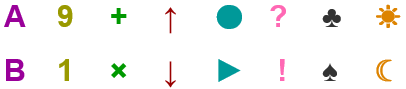
\includegraphics[scale=2]{papers/images_behavior_research_methods/Features8.png}
	\caption{
	% Pictured above are the features, the visual representation of the positive and negative values of the propositional variables. The upper row represents positive values of the propositional variables, while the lower row represents their negation.
	En la imagen de arriba se muestran las características, la representación visual de los valores positivos y negativos de las variables proposicionales. La fila superior representa valores positivos de las variables proposicionales, mientras que la fila inferior representa su negación.}
	\label{Figure:references}
\end{center}
\end{figure}


% \paragraph{Elements (boxes)\textemdash valuations.} A valuation over the propositional variables is visually represented as a square/box with the values (icons) of all propositional variables set at random positions inside the square. We call such representation an `element' (see Figure~\ref{Figure:element} for an example of such an element). The reason for choosing this representation is to avoid directional biases that could influence learning, and to exclude ordering and other operators from the language of thought (see \S\ref{Experiment_design} for more details). 
% Each time an element is shown (in particular, within the loop in the training-feedback) a new random position is chosen for the propositional features inside it.
\paragraph{Elementos (cajas)\textemdash valuaciones.} Una valuación sobre las variables proposicionales se representa visualmente como un cuadrado/caja con los valores (iconos) de todas las variables proposicionales colocadas en posiciones aleatorias dentro de la caja. Llamamos a esta representación un `elemento' (ver Figura~\ref{Figure:element} para ver un ejemplo de tal elemento). La razón para elegir esta representación es evitar sesgos direccionales que podrían influir en el aprendizaje y excluir el orden y otros operadores del lenguaje del pensamiento (consultar \S\ref{Experiment_design} para obtener más detalles).
Cada vez que se muestra un elemento (en particular, dentro del ciclo en la etapa de entrenamiento-{\em feedback}) se elige una nueva posición aleatoria para las características proposicionales dentro de él.


\begin{figure}[h!] 
\begin{center}
    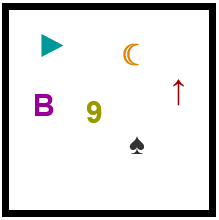
\includegraphics[scale=0.6]{papers/images_behavior_research_methods/BordeNeutro.PNG}
	\caption{
	% An element. This box containing features is the visual representation of a valuation over six propositional variables. Here the box appears with a neutral border, but boxes in the experiment always appear with a border that denotes whether they are positive or negative examples. The position of the symbols is irrelevant for the concepts, and is randomly assigned.
	Un elemento. Esta caja que contiene características es la representación visual de una valuación sobre seis variables proposicionales. Aquí la caja aparece con un borde neutro, pero las cajas del experimento siempre aparecen con un borde que denota si son ejemplos positivos o negativos. La posición de los símbolos es irrelevante para los conceptos y se asigna al azar.}
	\label{Figure:element} 
\end{center}
\end{figure}


% \paragraph{Undetermined concepts\textemdash sets of positive/negative valuations.}\label{IncompleteConcepts} The concept shown in the learning stage of a trial corresponds to two non-overlapping sets of valuations, and these two sets do not cover all possible valuations. This is represented as a sequence of `in' and `out' elements, with no information given on elements that are not shown.  At the learning stage, shown `in' elements (positive examples) are represented as a green box and shown `out' elements (negative examples) as a red box. See Figure~\ref{Figure:training} for an example of a tagged sequence of elements used in the learning stage. Each time the concept is presented, we shuffle the order in which their positive and negative examples are shown, but always presenting all positive examples first (also, each valuation is assigned new random positions for the features inside the corresponding box). 
\paragraph{Conceptos indeterminados\textemdash conjuntos de valuaciones positivas/negativas.} \label{IncompleteConcepts} El concepto que se muestra en la etapa de aprendizaje de una prueba corresponde a dos conjuntos de valuaciones que no se superponen, y estos dos conjuntos no cubren todas las valuaciones posibles. Esto se representa como una secuencia de elementos `adentro' y `afuera', sin información sobre los elementos que no se muestran. En la etapa de aprendizaje, los elementos `adentro' (ejemplos positivos) se representan como una caja con borde verde y los elementos `afuera (ejemplos negativos) como una caja con borde rojo. Consultar la Figura~\ref{Figure:training} para ver un ejemplo de una secuencia etiquetada de elementos utilizados en la etapa de aprendizaje. Cada vez que se presenta el concepto, barajamos el orden en el que se muestran sus ejemplos positivos y negativos, pero siempre presentando todos los ejemplos positivos primero (además, a cada valuación se le asignan nuevas posiciones aleatorias para las características dentro de la caja correspondiente).

\begin{figure}[h!] 
\begin{center}
    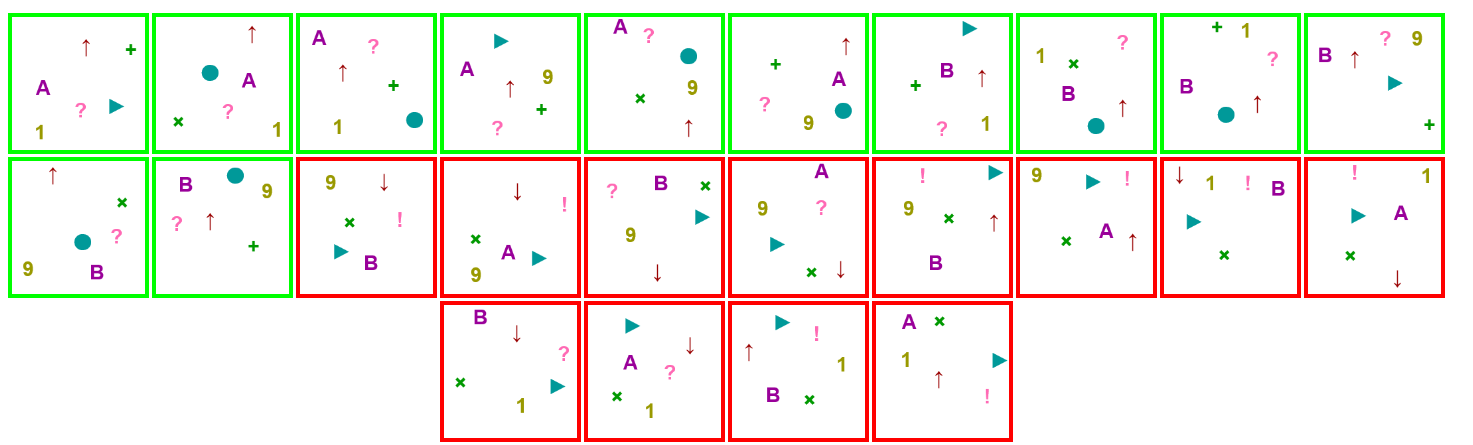
\includegraphics[scale=0.35]{papers/images_behavior_research_methods/Learning.PNG}
	\caption{
	% A sequence of positive and negative examples in a learning stage, corresponding to Trial 1.  A green border informs the participant that the element belongs to the concept, while a red-bordered one informs that it does not belong to the concept. In this case, the examples could be explained as either `boxes containing both an upwards pointing arrow and a question mark' or as `boxes that contain a circle or a plus sign', but note that these two rules determine different concepts over the complete set of possible elements.
	Una secuencia de ejemplos positivos y negativos en una etapa de aprendizaje, correspondiente a la Prueba 1. Un borde verde informa al participante que el elemento pertenece al concepto, mientras que un borde rojo informa que no pertenece al concepto. En este caso, los ejemplos podrían explicarse como `cajas que contienen una flecha que apunta hacia arriba y un signo de interrogación' o como `cajas que contienen un círculo o un signo más', pero hay que tener en cuenta que estas dos reglas determinan conceptos diferentes sobre el conjunto completo de posibles elementos.}
	\label{Figure:training}
\end{center}
\end{figure}

% \paragraph{(Hidden) concepts\textemdash formulas.}
% Over the full set of valuations, a concept is simply the set of valuations that positively describe it. The two hidden concepts for each trial correspond to the valid and minimal generalizations that can be made from the incomplete concepts. They can be described as the semantics of the two propositional formulas (rules) that can be used to explain the incomplete concept (see Table~\ref{trial_table}); while these rules coincide over the incomplete universe shown in the learning stage, they differ over the set of all valuations. For more details, recall the beginning of \S\ref{Subsec:ExperimentFlow} and its Item~\ref{item:LearningStage}. For technical details, see \S\ref{Sec:MainTheoremConcept}.
\paragraph{Conceptos (ocultos)\textemdash fórmulas.}
Sobre el conjunto completo de valuaciones, un concepto es simplemente el conjunto de valuaciones que lo describen positivamente. Los dos conceptos ocultos para cada prueba corresponden a las generalizaciones válidas y mínimas que se pueden hacer a partir de los conceptos incompletos. Pueden describirse como la semántica de las dos fórmulas proposicionales (reglas) que pueden usarse para explicar el concepto incompleto (ver Tabla~\ref{trial_table}); si bien estas reglas coinciden en el universo incompleto que se muestra en la etapa de aprendizaje, difieren en el conjunto de todas las valuaciones. Para obtener más detalles, recuerde el comienzo de \S\ref{Subsec:ExperimentFlow} y su Item~\ref{item:LearningStage}. Para obtener detalles técnicos, consultar \S\ref{Sec:MainTheoremConcept}.

\bigskip

% In Table~\ref{tab:glosario} we summarize the main logical terminology used to define formal semantics, and its representational counterpart adopted in our experimental setup.
En la Tabla~\ref{tab:glosario} resumimos la principal terminología lógica usada para definir la semántica formal, y su contraparte representacional adoptada en nuestra configuración experimental.

\widesanti{Parte (no toda) de esta tabla puede ser mandada al primer capítulo, dado que comparte mucho con el paper de PRE. habría que unificar nomenclatura entre PRE y BRM.}
\begin{table}[]
\begin{tabular}{c|c}
{\bf Terminología matemática}
&
{\bf Terminología representacional}
\\\hline
\begin{minipage}[t]{0.45\textwidth}
% {\bf Valuation}: a tuple $\overline v=(v_1,\dots,v_n)$ where each $v_i$ is 0 or 1. 
{\bf Valuación}: una tupla $\overline v=(v_1,\dots,v_n)$ donde cada $v_i$ es 0 o 1. 
\end{minipage}
& 
\begin{minipage}[t]{0.45\textwidth}
% {\bf Element}: a square with $n$ symbols inside (see Figure~\ref{Figure:element}). There is an implicit coding shown in  Figure~\ref{Figure:references} (for example, $v_1=1$ is represented by a `A' and  $v_1=0$ is represented by an `B', $v_3=1$ is represented by a `$+$' and  $v_3=0$ is represented by a `$\times$', and so on). 
{\bf Elemento}: una caja con $n$ símbolos dentro (ver Figura~\ref{Figure:element}). Hay un código implícito en la Figura~\ref{Figure:references} (por ejemplo, $v_1=1$ se representa por una `A' y  $v_1=0$ se representa por una `B', $v_3=1$ se representa por un `$+$' y  $v_3=0$ se representa por un `$\times$', y así sucesivamente). 

\end{minipage} 
\\\hline
\begin{minipage}[t]{0.45\textwidth}
% {\bf Propositional variable}: $p_i$ takes value $v_i$ under valuation $\overline v=(v_1,\dots,v_n).$
{\bf Variable proposicional}: $p_i$ toma el valor $v_i$ bajo la valuación $\overline v=(v_1,\dots,v_n).$
\end{minipage}
&
\begin{minipage}[t]{0.45\textwidth}
% {\bf Feature}: $p_i$ is represented, via the implicit coding, by one of the pairs of Figure~\ref{Figure:references} within an element representing $\overline v$.
{\bf Característica}: $p_i$ se representa, vía la codificación implícita, por uno de los pares de la Figura~\ref{Figure:references} dentro de un elemento que representa $\overline v$.
\end{minipage}
\\\hline
\begin{minipage}[t]{0.45\textwidth}
% {\bf Concept}: a set $U$ of valuations representing the `positive' ones (for example, $C_1$ in Figure \ref{fig:twoconcepts}). Notice that the negative valuations are just all valuations not in~$U$.\\
{\bf Concepto}: un conjunto $U$ de valuaciones que representa aquellas que son `positivas' (por ejemplo, $C_1$ en la Figura \ref{fig:twoconcepts}). Notar que las valuaciones negativas son simplemente todas las valuaciones que no están en~$U$.\\

% Observe that any concept $U$ has a corresponding minimal {\bf formula/rule} $\varphi_U$ that characterizes it (i.e.\ $\varphi_U$ is true over the valuations in $U$, and is false over the complement of $U$). 
Observar que cualquier concepto $U$ tiene una correspondiente {\bf formula/regla} minimal $\varphi_U$ que la caracteriza (es decir, $\varphi_U$ es verdadera para las valuaciones en $U$, y es falsa sobre el complemento de $U$). 
\end{minipage}&
\begin{minipage}[t]{0.45\textwidth}
% {\bf Concept}: any categorization that divides the space of all possible elements in either positive (all those elements that belong to $U$) or negative (elements that do not belong to $U$). 
{\bf Concepto}: cualquier categorización que divida el espacio de todos los elementos posibles en positivos (todos aquellos elementos que pertenecen a $ U $) o negativos (elementos que no pertenecen a $ U $).
\end{minipage}
\\\hline
\begin{minipage}[t]{0.45\textwidth}
% {\bf Undetermined concept}: 
% a pair $\langle U,V\rangle$ of sets of valuations representing the `positive' and `negative' ones respectively such that $U\cap V=\emptyset$ and $U\cup V$ is not the set of all valuations (for example, the pair $\langle C_1\cap C_2, \overline{C_1\cup C_2}\rangle$ in Figure \ref{fig:twoconcepts}).\\

{\bf Concepto indeterminado}:
un par $ \langle U, V \rangle $ de conjuntos de valuaciones que representan los valores `positivos' y `negativos' respectivamente, de modo que $ U \cap V = \emptyset $ y $ U \cup V $ no es el conjunto de todas las valuaciones (por ejemplo, el par $ \langle C_1 \cap C_2, \overline {C_1 \cup C_2} \rangle $ en la Figura \ref{fig:twoconcepts}). \\

% Observe that an undetermined concept $\langle U,V\rangle$ can be generalized in more than one way by (minimal) formulas $\varphi_1$ and $\varphi_2$ such that {\em a)} $\varphi_i$ ($i=1,2$) is true over all valuations in $U$, and false over all valuations on $V$, and {\em b)} the set {\em all} of positive valuations where $\varphi_1$ is true is different from the set of {\em all} valuations where $\varphi_2$ is true. For example, the undetermined concept shown in each trial $i$ of the experiment can be generalized via the two corresponding minimal formulas $\varphi^i_1$ and $\varphi^i_2$ shown in Table~\ref{trial_table}.
Observar que un concepto indeterminado $ \langle U, V \rangle $ puede generalizarse de más de una forma mediante fórmulas (mínimas) $ \varphi_1 $ y $ \varphi_2 $ tales que {\em a)} $ \varphi_i $ ($ i = 1,2 $) es verdadera en todas las valuaciones en $ U $, y falsa en todas las valuaciones en $ V $, y {\em b)} el conjunto de {\em todas} las valuaciones positivas donde $ \varphi_1 $ es verdadera es diferente del conjunto de {\em todas} las valuaciones donde $ \varphi_2 $ es verdadera. Por ejemplo, el concepto indeterminado que se muestra en la $ i $-ésima prueba del experimento se puede generalizar mediante las dos fórmulas mínimas correspondientes $ \varphi^i_1 $ y $ \varphi^i_2 $ que se muestran en la Tabla~\ref{trial_table}.
\end{minipage}
&
\begin{minipage}[t]{0.45\textwidth}
% {\bf Undetermined concept}: a sequence of positive elements (green border)  representing $U$, and negative elements (red border) representing $V$ (see Figure~\ref{Figure:training} for an example). Importantly, $U$ and $V$ do not cover the full universe of possibilities spanned by the features.
{\bf Concepto indeterminado}: una secuencia de elementos positivos (borde verde) que representan $ U $ y elementos negativos (borde rojo) que representan $ V $ (consultar la Figura~\ref{Figure:training} para un ejemplo). Es importante destacar que $ U $ y $ V $ no cubren todo el universo de posibilidades que abarcan las funciones.\end{minipage}
\end{tabular}
% \caption{Terminology used for explaining the formal semantics of Boolean logic both in mathematical terms and in the representational terms used in the experiment.}
% \label{tab:glosario}
\caption {Terminología utilizada para explicar la semántica formal de la lógica booleana tanto en términos matemáticos como en los términos de representación utilizados en el experimento.}
\label{tab:glosario}
\end{table}




% \subsection{Details of the experiment's structure} \label{FullExperimentDescription} 
\subsection{Detalles de la estructura del experimento} \label{FullExperimentDescription} 

% As we explain in Section~\ref{Section:Experiment}, each instance of the experiment consists of 6 trials where the participants must learn a concept from an incomplete universe. The presented positive and negative examples are such that there are exactly two minimal rules (up to logical equivalence) in propositional logic that {\em 1)} are consistent explanations for the shown examples; {\em 2)} use disjoint sets of variables from each another; and {\em 3)} any rule consistent with the examples must use a superset of the set of features of at least one of these minimal rules. This experimental setup will allow us to distinguish which of these rules best represents the way that the participant learned the concept. See \S\ref{Sec:MainTheoremConcept} for technical details.
Como explicamos en la Sección~\ref{Section:Experiment}, cada instancia del experimento consta de 6 pruebas en las que los participantes deben aprender un concepto de un universo incompleto. Los ejemplos positivos y negativos presentados son tales que hay exactamente dos reglas mínimas (salvo equivalencia lógica) en la lógica proposicional que {\em 1)} son explicaciones consistentes para los ejemplos mostrados; {\em 2)} usan conjuntos de variables disjuntos entre sí; y {\em 3)} cualquier regla consistente con los ejemplos debe usar un superconjunto del conjunto de características de al menos una de estas reglas mínimas. Esta configuración experimental nos permitirá distinguir cuál de estas reglas representa mejor la forma en que el participante aprendió el concepto. Consultar \S\ref{Sec:MainTheoremConcept} para los detalles técnicos.


% Observe that merely asking the participant to select already seen elements does not give us any obvious insight into the internal process that derived into the learning of the concept; even if they internalized the concept using one of the two rules, it would remain uncertain which one they used, as both rules have the same semantics over the shown universe. In order to distinguish between these two cases, we use a generalization stage where previously unseen elements of the universe are shown, and the participant must select those that they believe belong to the concept. Of these new elements, some are consistent with only one of the rules, and other are consistent only with the other rule\footnote{The Trial 6 is an exception, and has an element that is consistent with both rules.}. Furthermore, immediately afterwards we ask for a written explanation of what characteristics the participant thinks describe the  concept.
Observar que el simple hecho de pedirle al participante que seleccione elementos ya vistos no nos da una idea obvia del proceso interno que derivó en el aprendizaje del concepto; incluso si internalizaran el concepto usando una de las dos reglas, sería incierto cuál usaron, ya que ambas reglas tienen la misma semántica sobre el universo mostrado. Para distinguir entre estos dos casos, utilizamos una etapa de generalización donde se muestran elementos del universo nunca antes vistos, y el participante debe seleccionar aquellos que crea que pertenecen al concepto aprendido. De estos nuevos elementos, algunos son consistentes con solo una de las reglas, y otros son consistentes solo con la otra regla\footnote{La Prueba 6 es una excepción y tiene un elemento que es consistente con ambas reglas.}. Además, inmediatamente después pedimos una explicación por escrito de las características que el participante cree que describen el concepto.

% Structurally, the experiment begins with the (hidden) assignment of the participant to one of two groups X or Y (see Table~\ref{trial_table}) and the exposition to a page with instructions. 
% Afterwards, there are 6 trials with the following structure: they begin with a learning stage; they continue to a training stage where they get feedback if they fail to correctly select the elements that belong to the concept; a generalization stage where they must choose between elements of the universe that were not shown previously; and, in all but the last trial, a stage where the participants can rest between trials.
Estructuralmente, el experimento comienza con la asignación (oculta) del participante a uno de los dos grupos X o Y (ver Tabla~\ref{trial_table}) y la exposición a una página con instrucciones.
Posteriormente, se realizan 6 pruebas con la siguiente estructura: comienzan con una etapa de aprendizaje; continúan a una etapa de aprendizaje donde reciben {\em feedback} si no seleccionan correctamente los elementos que pertenecen al concepto; una etapa de generalización donde deben elegir entre elementos del universo que no fueron mostrados previamente; y, en todos menos en la última prueba, una etapa en la que los participantes pueden descansar entre ensayos.

% In what follows, we describe each stage of the experiment plus the introductory page, with a greater detail than that of \S\ref{Subsec:ExperimentFlow}.
A continuación, describimos cada etapa del experimento más la página de introducción, con mayor detalle que en \S\ref{Subsec:ExperimentFlow}.

% \subsubsection{Introduction and explanation}
\subsubsection{Introducción y explicación}

% This is the page that subjects are shown at the beginning of the experiment. It describes the main task they will be asked to perform: that of learning from examples to distinguish what kind of `boxes' belong to a certain concept. These elements are represented as a collection of 6 symbols, no more than one from a same pair. It is also informed that the position of the symbols does not matter. See Figure~\ref{Figure:element} for an example element.
Esta es la página que se muestra a los sujetos al comienzo del experimento. Describe la tarea principal que se les pedirá que realicen: la de aprender de ejemplos para distinguir qué tipo de `cajas' pertenecen a un determinado concepto. Estos elementos se representan como una colección de 6 símbolos, no más de uno de un mismo par. También se le informa que la posición de los símbolos no importa. Consultar la Figura~\ref{Figure:element} para ver un elemento de ejemplo.

% When the subject indicates they have finished reading the instructions, they are sent to a fullscreen page with three multiple-choice questions whose purpose is to verify that the participant has understood the instructions; if they miss some answer, they are returned to the previous page and the cycle is repeated until they succeed.
Cuando el sujeto indica que ha terminado de leer las instrucciones, se lo envía a una página de pantalla completa con tres preguntas de opción múltiple cuyo propósito es verificar que el participante ha entendido las instrucciones; si se equivoca en alguna respuesta, vuelve a la página anterior y el ciclo se repite hasta que lo consiguen.

% If the participant answers correctly, they are now ready to begin, and the phases~\S\ref{Subsection:learning}, \S\ref{Subsection:training}, and \S\ref{Subsection:generalization} are then entered sequentially for each of the 6 trials.
Si el participante responde correctamente, está listo para comenzar, y se ingresan a las fases~\S\ref{Subsection:learning}, \S\ref{Subsection:training}, y \S\ref{Subsection:generalization} secuencialmente para cada uno de los 6 ensayos.

% \subsubsection{The learning phase}\label{Subsection:learning}
\subsubsection{La fase de aprendizaje}\label{Subsection:learning}

% In this phase of a Trial $i$, the participant is shown a set $S^i \subsetneq U^i$, a proper subset of elements from the current universe. Each universe syntactically corresponds to all the combinations of truth values for 6 propositional variables taken from the set $\{\varA, \varB, \varC, \varD, \varE, \varF, \varG, \varH\}$, thus spawning a set $U^i$ of 64 elements. On the semantic side we call `features' the visual representations of the propositional variables, and these representations remain fixed through the experiment (recall Figure~\ref{Figure:references}).
En esta fase de una Prueba $ i $, al participante se le muestra un conjunto $ S^i \subsetneq U^i $, un subconjunto adecuado de elementos del universo actual. Cada universo corresponde sintácticamente a todas las combinaciones de valores de verdad para 6 variables proposicionales tomadas del conjunto $\{\varA, \varB, \varC, \varD, \varE, \varF, \varG, \varH\}$, por lo tanto generando un conjunto $ U^i $ de 64 elementos. Del lado semántico, llamamos `características' a las representaciones visuales de las variables proposicionales, y estas representaciones permanecen fijas durante el experimento (recordar la Figura~\ref{Figure:references}).

% The elements of $S^i$ are shown as boxes, some of which have green border (denoting a positive example, that the element belongs to the concept), while the rest have red borders (denoting a negative example, that they do not belong).The green-bordered boxes are shown first, with the red-bordered ones appearing after the last box with green border. See Figure~\ref{Figure:training} for an example learning set. 
Los elementos de $ S^i $ se muestran como cajas, algunas de las cuales tienen borde verde (que denota un ejemplo positivo, es decir que el elemento pertenece al concepto), mientras que el resto tiene bordes rojos (que denota un ejemplo negativo, es decir que no lo hacen). Las cajas de borde verde se muestran primero, y las de borde rojo aparecen después de la última caja con borde verde. Consultar la Figura~\ref{Figure:training} para ver un ejemplo de conjunto de aprendizaje.

% If the graphical representations are abstracted away to the underlying basic structure, there are two propositional rules $\varphi^i_1$ and $\varphi^i_2$ (of minimum length in their class of logically equivalent rules, see Table~\ref{trial_table}) whose semantics correctly classify the positive and negative examples shown. If we call $C^i_1, C^i_2$ the sets of valuations that satisfy $\varphi^i_1, \varphi^i_2$, respectively, we have that $S^i = (C^i_1 \cap C^i_2) \cup \overline{(C^i_1 \cup C^i_2)}$. The rules $\varphi^i_1, \varphi^i_2$ use at most\footnote{The rules that are actually `learnable' use exactly 2 propositional variables.} 3 of the 6 propositional variables available in $U^i$, and the two rules do not have propositional variables in common. 
Si las representaciones gráficas se abstraen de la estructura básica subyacente, hay dos reglas proposicionales $ \varphi^i_1 $ y $ \varphi^i_2 $ (de longitud mínima en su clase de reglas lógicamente equivalentes, consultar la Tabla~\ref{trial_table}) cuya semántica clasifica correctamente los ejemplos positivos y negativos mostrados. Si llamamos $ C^i_1, C^i_2 $ a los conjuntos de valuaciones que satisfacen $ \varphi^i_1, \varphi^i_2 $, respectivamente, tenemos que $ S^i = (C^i_1 \cap C^i_2) \cup \overline {(C^i_1 \cup C^i_2)} $. Las reglas $ \varphi^i_1, \varphi^i_2 $ usan a lo sumo\footnote{Las reglas que son realmente `aprendibles' usan exactamente 2 variables proposicionales.} 3 de las 6 variables proposicionales disponibles en $ U^i $, y las dos reglas no tienen variables proposicionales en común.

% When the participant believes they have learned which elements belong to the concept, they can click a button to proceed to the next stage.
Cuando el participante cree que ha aprendido qué elementos pertenecen al concepto, puede hacer clic en un botón para pasar a la siguiente etapa.

% \subsubsection{The training\textendash feedback phase}\label{Subsection:training}
\subsubsection{La fase de entrenamiento\textendash{\em feedback}}\label{Subsection:training}

% In this phase, the participant is shown a random rearrangement of $S^i$, with all the elements now surrounded by a red-bordered square. The subject must click exactly those elements (if any) they believe belong to the concept \textemdash changing them to a dotted green border (see Figure~\ref{Figure:ElementSquares})\textemdash\ and then has to click a button to submit their choice.
En esta fase, al participante se le muestra un reordenamiento aleatorio de $S^i $, con todos los elementos ahora rodeados por un cuadrado con borde rojo. El sujeto debe hacer clic exactamente en esos elementos (si los hay) que cree que pertenecen al concepto \textemdash cambiándolos a un borde verde punteado (ver Figura~\ref{Figure:ElementSquares})\textemdash \ y luego debe hacer clic en un botón para enviar su elección.

\begin{figure}[h!] 
\begin{center}
    	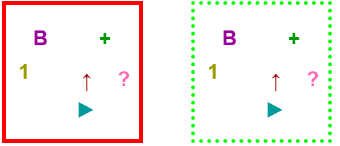
\includegraphics[scale=0.6]{papers/images_behavior_research_methods/SelectionSeparadosIguales.png}
	\caption{
	% An unselected element, to the left, is represented by solid red borders. The same element in a selected state, to the right, is indicated by dotted green borders.
	Un elemento no seleccionado, a la izquierda, está representado por bordes rojos sólidos. El mismo elemento en un estado seleccionado, a la derecha, se indica con bordes verdes punteados.}
	\label{Figure:ElementSquares}
\end{center}
\end{figure}

% If their selection  is  incorrect, the participant is shown which elements they misclassified (either by clicking them incorrectly or by failing to click them, see Figure~\ref{Figure:Misclassifications}). When they click a button to continue, they restart this stage (with a fresh randomization).
Si su selección es incorrecta, se le muestra al participante qué elementos clasificaron erróneamente (ya sea haciendo clic en ellos incorrectamente o no haciendo clic en ellos, consulte la Figura~\ref{Figure:Misclassifications}). Cuando hacen clic en un botón para continuar, reinician esta etapa (con una nueva mezcla aleatoria en la posición de las cajas y los símbolos dentro de ellas).

\begin{figure}[h!] 
\begin{center}
    	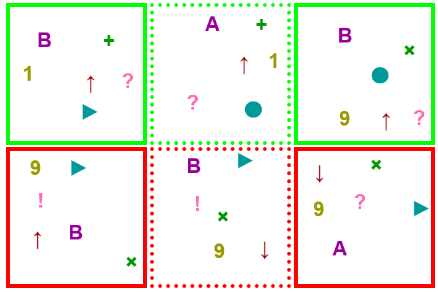
\includegraphics[scale=0.5]{papers/images_behavior_research_methods/FeedBack2SeleccionParcial.PNG}
	\caption{
	% A partial section of the feedback resulting from a wrong selection. A solid green border means that the box was correctly selected as belonging to the concept. A solid red border means that it was correctly left unselected, meaning that it did not belong to the concept. A dotted green border means the box belongs to the concept but was not selected, and a dotted red border means that the box does not belong to the concept but was selected.
	Una sección parcial del {\em feedback} resultante de una selección incorrecta. Un borde verde sólido significa que la casilla se seleccionó correctamente como perteneciente al concepto. Un borde rojo sólido significa que se dejó sin seleccionar correctamente, lo que significa que no pertenecía al concepto. Un borde verde punteado significa que la caja pertenecía al concepto pero no fue seleccionado, y un borde rojo punteado significa que la caja no pertenecía al concepto pero fue seleccionado.}
	\label{Figure:Misclassifications}
\end{center}
\end{figure}

% When the participant finally makes the correct selection, they continue to the next phase. 
Cuando el participante finalmente hace la selección correcta, pasa a la siguiente fase.

% \subsubsection{The generalization phase}\label{Subsection:generalization}
\subsubsection{La fase de generalización}\label{Subsection:generalization}

% In this phase, the participant is shown a subset of $U^i \backslash S^i$ (namely, in $(C^i_1 \cup C^i_2) \backslash (C^i_1 \cap C^i_2)$), that is, a selection of elements that were \emph{not} present in the learning phase (hence nor in the training phase). The participant must classify which of these elements they think belong to the concept. The participant does not receive feedback on the choices they make here. Except for the sixth trial, part of these elements satisfy the rule $\varphi^i_1 \land \lnot \varphi^i_2$, while the rest satisfy $\varphi^i_2 \land \lnot \varphi^i_1$. Thus \textemdash assuming the participant learned the concept via a process akin to a representation of one of the two rules\textemdash\, this phase crucially serves to distinguish which rule they have learned, if any.
En esta fase, se muestra al participante un subconjunto de $U^i \backslash S^i $ (o sea, $(C^i_1 \cup C^i_2) \backslash (C^i_1 \cap C^i_2) $), es decir, una selección de elementos que \emph {no} estaban presentes en la fase de aprendizaje (por tanto, tampoco en la de aprendizaje). El participante debe clasificar cuáles de estos elementos cree que pertenecen al concepto. El participante no recibe comentarios sobre las elecciones que hace aquí. Excepto por la sexta prueba, parte de estos elementos satisfacen la regla $\varphi^i_1 \land \lnot \varphi^i_2$, mientras que el resto satisface $\varphi^i_2 \land \lnot \varphi^i_1$. Por lo tanto, \textemdash asumiendo que el participante aprendió el concepto a través de un proceso similar a la representación de una de las dos reglas\textemdash\, esta fase sirve de manera crucial para distinguir qué regla ha aprendido, si es que ha aprendido alguna.

% After this selection, the participant is asked to submit a written explanation of what characteristics they think constitute the concept. This written explanation serves as an additional validation of whether they are thinking in a way describable by propositional logic according to our assumptions, or if rather they are using other methods (memorization, pen and paper, screenshots, other logics or formalisms, etc.). 
Después de esta selección, se solicita al participante que presente una explicación por escrito de lo que cree que define al concepto. Esta explicación escrita sirve como una validación adicional de si están pensando de una manera descriptible por lógica proposicional según nuestros supuestos, o si más bien están usando otros métodos (memorización, lápiz y papel, capturas de pantalla, otras lógicas o formalismos, etc.).

% \subsection{Notes on the experiment design}\label{Experiment_design}
\subsection{Notas sobre el diseño del experimento}\label{Experiment_design}


% The elements, universes, and rules that constitute our experiment are devised in terms of propositional logic. However, it is important to be careful with the semantics, i.e.\ the way elements are actually shown to the participants. We have to avoid giving more salience to the semantics of a propositional variable over the others, and it is imperative to select the semantics of variables in a way such that they do not share characteristics that might escape our propositional grammar: for example, if the propositional variables were represented as circles that can be distinctly colored or not, it would be quite natural to assume that counting colored or uncolored circles could provide information, but this option is not considered in a theoretical design that assumes only propositional operators to describe rules. A related consideration is that we must also avoid introducing other regularities extraneous to the propositional formulation: if the images corresponding to all propositional variables are always shown in a straight line in the same order, salience effects might appear \textit{even if }we avoid semantics that become more expressive thanks to the ordered nature of the represented variables (such as with descriptions of the form \textit{the first and last elements are of the same size}).
Los elementos, universos y reglas que constituyen nuestro experimento están diseñados en términos de lógica proposicional. Sin embargo, es importante ser cuidadosos con la semántica, es decir, la forma en que los elementos se muestran realmente a los participantes. Tenemos que evitar dar más prominencia a la semántica de una variable proposicional sobre las demás, y es imperativo seleccionar la semántica de las variables de tal manera que no compartan características que puedan escapar a nuestra gramática proposicional: por ejemplo, si las variables proposicionales se representaron como círculos que pueden tener distintos colores o no, sería bastante natural suponer que contar círculos coloreados o no coloreados podría proporcionar información, pero esta opción no se considera en un diseño teórico que asume solo operadores proposicionales para describir reglas. Una consideración relacionada es que también debemos evitar introducir otras regularidades ajenas a la formulación proposicional: si las imágenes correspondientes a todas las variables proposicionales se muestran siempre en línea recta en el mismo orden, los efectos de prominencia pueden aparecer \textit{incluso si} evitamos semánticas que se vuelven más expresivas gracias a la naturaleza ordenada de las variables representadas (como con descripciones de la forma \textit{el primer y último elemento son del mismo tamaño}).\santi{aca podes referenciar a los semáforos de PRE y decir que este diseño lo supera}


% \paragraph{Building adequate semantic representations for our logic.}
\paragraph{Construyendo representaciones semánticas adecuadas para nuestra lógica.}

% Taking these precautions into account, we choose to match each propositional variable with a particular image or figure, whose position in a square would be randomized (but avoiding superpositions). It  is harder to decide exactly what would be the matching, but our final decision consists in matching each propositional variable with a set of two related Unicode characters (such as a triangle when the variable is $0$, and a circle otherwise). See Figure~\ref{Figure:references} for the exact representations. We take care to choose different types of characters for different variables: having $A,B$ for $\varA$ and $Y,Z$ for $\varE$ is out as a possibility, since it naturally  introduces counting of the type `there is no more than 1 letter' and the like. Of course, this process is not fail-safe, as there are countless possible semantics associations that could introduce extra-propositional grammar into the experiment. But we try to minimize the chance that this happens easily or naturally, and we use the written explanation stage as a way to catch these exceptions if they occur\footnote{In the end, they did not occur. See \S\ref{Sec:ExclusionCriteria}.}. 
Teniendo en cuenta estas precauciones, optamos por hacer coincidir cada variable proposicional con una imagen o figura en particular, cuya posición en un cuadrado sería aleatoria (pero evitando superposiciones). Es difícil decidir exactamente cuál sería la mejor coincidencia de variable a imagen, pero nuestra decisión final consiste en hacer coincidir cada variable proposicional con un conjunto de dos caracteres Unicode relacionados (como un triángulo cuando la variable es $ 0 $ y un círculo en caso contrario). Ver la Figura~\ref{Figure:references} para las representaciones exactas. Nos encargamos de elegir diferentes tipos de caracteres para diferentes variables: tener $ A, B $ para $ \varA $ y $ Y, Z $ para $ \varE $ es una posibilidad, ya que naturalmente introduce el conteo del tipo `no hay más de 1 letra' y similares. Por supuesto, este proceso no es completamente seguro, ya que existen innumerables asociaciones semánticas posibles que podrían introducir gramáticas extra-proposicionales en el experimento. No obstante, tratamos de minimizar la posibilidad de que esto suceda fácil o naturalmente, y usamos la etapa de explicación escrita como una forma de detectar estas excepciones si ocurriesen \footnote {Al final, no ocurrieron. Consultar \S\ref{Sec:ExclusionCriteria}.}.

% Finally, to minimize possible salience effects from showing symbols that could have (despite our intentions to the contrary) different levels of conspicuousness, we randomize on a per-participant basis the assignment between pairs of symbols and propositional variables (but we do not randomize  the assignment to the positive or negative value of a variable; the same Unicode characters  are  always positive in all randomizations, or always negative).
Finalmente, para minimizar los posibles efectos de prominencia de mostrar símbolos que podrían tener (a pesar de nuestras intenciones en la dirección contraria) diferentes niveles de notoriedad, aleatorizamos por participante la asignación entre pares de símbolos y variables proposicionales (pero no aleatorizamos la asignación al valor positivo o negativo de una variable; los mismos caracteres Unicode son siempre positivos en todas las aleatorizaciones, o siempre negativos).

% \paragraph{Ordering of positive and negative examples.}
\paragraph{Orden de ejemplos positivos y negativos.}

% As mentioned before, in the learning stage we shuffle the order in which their positive and negative examples are shown, but always presenting all positive examples first. Also, the number of positive examples is smaller or equal to the number of negative examples for all concepts (see Table \ref{trial_table}). 
Como se mencionó anteriormente, en la etapa de aprendizaje cambiamos el orden en el que se muestran los ejemplos positivos y negativos, pero siempre presentando todos los ejemplos positivos primero. Además, el número de ejemplos positivos es menor o igual al número de ejemplos negativos para todos los conceptos (ver Tabla~\ref{trial_table}).

% The purpose of placing the positive examples first and having less positive examples than negative ones is to bias the participant into thinking of the concept by its positive formulation, instead of possibly thinking of a rule that would describe the negative examples, and then negating that rule to obtain the positive one. This becomes important when we want to reason about the ease of learning of different operators: the default assumption is that participants that correctly select positive examples of the concept are thinking the positive rule, which differs in its operator from the negative rule (by the De Morgan laws). 
El propósito de colocar los ejemplos positivos primero y tener menos ejemplos positivos que negativos es sesgar al participante para que piense en el concepto por su formulación positiva, en lugar de pensar posiblemente en una regla que describa los ejemplos negativos, y luego negar esa regla para obtener el positivo. Esto se vuelve importante cuando queremos razonar sobre la facilidad de aprendizaje de diferentes operadores: la suposición predeterminada es que los participantes que seleccionan correctamente ejemplos positivos del concepto piensan en la regla positiva, que difiere en su operador de la regla negativa (por las leyes de De Morgan).


% \section{Results}\label{Results}
\section{Resultados}\label{Results}


% \subsection{Hypothesis~\ref{Hip:AndOverOr}}\label{Results:AndOverOr}
\subsection{Hipótesis~\ref{Hip:AndOverOr}}\label{Results:AndOverOr}

% We asked whether the conjunction-disjunction bias (which is known to affect learning times in the case of a single explanation~\cite{bourne1970knowing}) also determines which features are used to describe a concept when two alternative explanations are consistent with the observed universe. In the first trial, the observed examples were consistent with $p_1 \vee p_2$ and with $p_3 \wedge p_4$. As explained in \S\ref{Subsec:ExperimentFlow}, in the generalization stage we can determine if participants explained the concept using $\{p_1,p_2\}$ or $\{p_3,p_4\}$. We found that 77 of the 100 participants attended to $\{p_3,p_4\}$, which corresponds to an explanation that uses a conjunction. 11 participants attended to $\{p_1,p_2\}$ (corresponding to the use of a disjunction for the explanation), and 12 participants selected examples in the generalization stage inconsistent with both $p_3 \wedge p_4$ and $p_1 \vee p_2$. To test the significance of this result, we performed a permutation test. Under the null hypothesis that participants randomly choose between explaining the concept using features $\{p_1,p_2\}$ and explaining it using $\{p_3,p_4\}$, the probability that 77 of the 100 participants attend to $\{p_3,p_4\}$ is $P<10^{-12}$. Thus we conclude that the observed difference is significant. 
Nos preguntamos si el sesgo de conjunción-disyunción (que se sabe que afecta los tiempos de aprendizaje en el caso de una explicación única~\cite{bourne1970knowing}) también determina qué características se usan para describir un concepto cuando dos explicaciones alternativas son consistentes con el universo observado. En la primera prueba, los ejemplos observados fueron consistentes con $ p_1 \vee p_2 $ y con $ p_3 \wedge p_4 $. Como se explica en \S\ref{Subsec:ExperimentFlow}, en la etapa de generalización podemos determinar si los participantes explicaron el concepto usando $ \{p_1, p_2 \} $ o $ \{p_3, p_4 \} $. Encontramos que 77 de los 100 participantes prestaron atención a $ \{p_3, p_4 \} $, que corresponde a una explicación que usa una conjunción. 11 participantes se enfocaron a $ \{p_1, p_2 \} $ (correspondiente al uso de una disyunción para la explicación), y 12 participantes seleccionaron ejemplos en la etapa de generalización inconsistentes con $ p_3 \wedge p_4 $ y $ p_1 \vee p_2$. Para probar la importancia de este resultado, realizamos una prueba de permutación. Bajo la hipótesis nula de que los participantes eligen aleatoriamente entre explicar el concepto usando las características $ \{p_1, p_2 \} $ y explicarlo usando $ \{p_3, p_4 \} $, la probabilidad de que 77 de los 100 participantes asistan a $ \{ p_3, p_4 \} $ es $ P <10^{-12} $. Por tanto, concluimos que la diferencia observada es significativa.

% Note that it is in principle possible that the participant learned the concept with a focus on negative examples ({\sf B}'s in Figure~\ref{fig:trials}) instead of on positive examples ({\sf A}'s in Figure~\ref{fig:trials}) (i.e. finding a correct explanation for the negative examples and then negating that rule to obtain an explanation for the positive examples). 
Hay que tener en cuenta que, en principio, es posible que el participante haya aprendido el concepto con un enfoque en ejemplos negativos ({\sf B}s en la Figura~\ref{fig:trial}) en lugar de en ejemplos positivos ({\ sfA}s en la Figura~\ref{fig:trial}) (es decir, encontrar una explicación correcta para los ejemplos negativos y luego negar esa regla para obtener una explicación para los ejemplos positivos).

% As we mention in \S\ref{Experiment_design}, we induced a bias to understand the concept in the appropriate way by first presenting the positive examples in the learning phase and by asking them to click on the positive ones in the training phase. We note, however, that 9 participants gave verbal explanations consistent with focusing on the negative examples. In this particular trial, a reverse interpretation is problematic since the negation of a conjunction corresponds to a disjunction, and the negation of the disjunction to a conjunction (i.e.\ $p\land q$ is logically equivalent to $\lnot(\lnot p\lor \lnot q)$). Thus, a more comprehensive analysis should take into account participants' verbal explanations in this trial. However, even considering the worst-case scenario in which these 9 participants were originally regarded as part of the `conjunction' group and they are now considered part of the `disjunction' group, the conjunction-disjunction bias is still significant ($P<10^{-7}$). We therefore conclude that, in this framework where multiple explanations are possible depending on the attended features, there is a bias favoring conjunctive explanations over disjunctive explanations. 
Como mencionamos en \S\ref{Experiment_design}, indujimos un sesgo para comprender el concepto de la manera adecuada presentando primero los ejemplos positivos en la fase de aprendizaje y pidiéndoles que hicieran clic en los positivos en la fase de entrenamiento. Sin embargo, observamos que nueve participantes dieron explicaciones verbales coherentes con el enfoque en los ejemplos negativos. En esta prueba en particular, una interpretación inversa es problemática ya que la negación de una conjunción corresponde a una disyunción, y la negación de la disyunción a una conjunción (es decir, $ p \land q $ es lógicamente equivalente a $ \lnot (\lnot p \lor \lnot q) $). Por lo tanto, un análisis más completo debe tener en cuenta las explicaciones verbales de los participantes en esta prueba. Sin embargo, incluso considerando el peor escenario en el que estos 9 participantes fueran considerados originalmente como parte del grupo de  `conjunción' y ahora se consideren parte del grupo de `disyunción', el sesgo de conjunción-disyunción sigue siendo significativo ($ P<10^{-7} $). Por lo tanto, concluimos que, en este marco donde son posibles múltiples explicaciones dependiendo de las características enfocadas, existe un sesgo que favorece las explicaciones conjuntivas sobre las explicaciones disyuntivas.

% \subsection{Hypothesis \ref{Hip:FeatureBiasStickiness}}\label{Results:FeatureBiasStickiness}
\subsection{Hipótesis \ref{Hip:FeatureBiasStickiness}}\label{Results:FeatureBiasStickiness}

% Most participants understood the concept in Trial 6 using the same features $\{p_7,p_8\}$ used to describe the concept in Trial~5, even when the logical structure of the rule was exactly the same independently of attending to $\{p_7,p_8\}$ or to $\{p_3,p_4\}$\footnote{As expected by our experiment design, 94 of the 100 participants understood the concept in Trial 5 using features $\{p_7,p_8\}$ (6 selected features with no clear rationale). Using features $\{p_7,p_8\}$ is indeed the only plausible way to learn the concept, given the high complexity of the alternative MDL15 formula. }. To show this, we study participants' choices in the generalization stage of Trial 6 (see Figure~\ref{fig:results1}). 
La mayoría de los participantes entendieron el concepto en la Prueba 6 usando las mismas características $ \{p_7, p_8 \} $ que se usaron para describir el concepto en la Prueba~5, incluso cuando la estructura lógica de la regla era exactamente la misma independientemente de prestar atención a $ \{ p_7, p_8 \} $ o $  \{p_3, p_4 \} $\footnote{Como se esperaba en el diseño de nuestro experimento, 94 de los 100 participantes entendieron el concepto en la Prueba 5 usando las características $ \{p_7, p_8 \} $ (6 características seleccionadas sin una justificación clara). Usar las características $ \{p_7, p_8 \} $ es de hecho la única forma plausible de aprender el concepto, dada la alta complejidad de la fórmula alternativa MDL15.}. Para mostrar esto, estudiamos las elecciones de los participantes en la etapa de generalización de la Prueba 6 (consultar la Figura~\ref {fig:results1}).

% Suppose that a participant is thinking of the rule $\lnot p_7 \land \lnot p_8$, thus they are only attending to features $\{p_7,p_8\}$ while ignoring the features $\{p_3,p_4\}$. Since $\{p_3,p_4\}$ are being ignored, the participant should mark those elements in which $\{p_7,p_8\}$ agrees with the rule $\lnot p_7 \land \lnot p_8$, irrespective of the values of $\{p_3,p_4\}$. That is, the participant should mark the elements with $\{p_3,p_4,p_7,p_8\}$ equal to $(0,0,\textbf{0,0})$, $(1,0,\textbf{0},\textbf{0})$, $(0,1,\textbf{0},\textbf{0})$ and $(1,1,\textbf{0},\textbf{0})$. These elements have $\{p_7,p_8\}$ equal to $(0,0)$ and `anything' for $\{p_3,p_4\}$. On the other hand, if the participant is thinking of the rule $p_3 \land \lnot p_7 \land \lnot p_8$, then she is attending to $\{p_3,p_7,p_8\}$, and she should mark $(\textbf{1},0,\textbf{0},\textbf{0})$ and $(\textbf{1},1,\textbf{0},\textbf{0})$. 
Supongamos que un participante está pensando en la regla $ \lnot p_7 \land \lnot p_8 $, por lo que solo está dirigiendo su atención a las características $ \{p_7, p_8 \} $ mientras ignora las características $ \{p_3, p_4 \} $. Dado que se ignoran $ \{p_3, p_4 \} $, el participante debe marcar aquellos elementos en los que $ \{p_7, p_8 \} $ está de acuerdo con la regla $ \lnot p_7 \land \lnot p_8 $, independientemente de los valores de $ \{p_3, p_4 \} $. Es decir, el participante debe marcar los elementos con $ \{p_3, p_4, p_7, p_8 \} $ igual a $ (0,0, \textbf {0, 0}) $, $ (1,0, \textbf { 0}, \textbf {0}) $, $ (0,1, \textbf {0}, \textbf {0}) $ y $ (1,1, \textbf {0}, \textbf {0}) $. Estos elementos tienen $ \{p_7, p_8 \} $ igual a $ (0,0) $ y `cualquier valor' por $ \{p_3, p_4 \} $. Por otro lado, si el participante está pensando en la regla $ p_3 \land \lnot p_7 \land \lnot p_8 $, entonces está atendiendo a $ \{p_3, p_7, p_8 \} $, y debe marcar $ ( \textbf {1}, 0, \textbf {0}, \textbf {0}) $ y $ (\textbf {1}, 1, \textbf {0}, \textbf {0}) $.

% In general, by studying which of the 7 examples shown in Figure~\ref{fig:results1} (left) the participant selects in the generalization phase, we can deduce which features they were attending to (Figure~\ref{fig:results1}, right). For example, all participants should mark the example with $\{p_3,p_4,p_7,p_8\}$ equal to $(1,1,0,0)$, since it is consistent with all the logical rules irrespective of which features are used. 
En general, al estudiar cuál de los 7 ejemplos que se muestran en la Figura~\ref{fig:results1} (izquierda) selecciona el participante en la fase de generalización, podemos deducir qué características estaban atendiendo (Figura~\ref{fig:results1 }, derecha). Por ejemplo, todos los participantes deben marcar el ejemplo con $ \{p_3, p_4, p_7, p_8 \} $ igual a $ (1,1,0,0) $, ya que es coherente con todas las reglas lógicas independientemente de las características son usadas.

% Indeed, as shown in Figure~\ref{fig:results1} (left), all participants selected this example. Although in practice the participant can select any of the 7 examples in the generalization stage, we found that all but five participants respected the rules of coherence illustrated in the previous paragraph. These 5 participants were `one example away' of respecting the rule, however, we leave them out of the feature stickiness analysis, but including them does not change our conclusions. We also excluded 6 participants that selected elements with no clear rationale in the previous trial, since they may not have used features $\{p_7,p_8\}$. However, including these participants (and assuming they did use $\{p_7,p_8\}$ in the previous trial) does not significantly change the results. In total, these two exclusions leaves 89 participants for this analysis. The grey lines in Figure~\ref{fig:results1} (left) show simulations of agents that randomly select one of the seven possible subsets of features, and then proceed to select the examples consistent with the logical rule using that features. Participants responses (black line) were biased towards explanations using $\{p_7,p_8\}$, as predicted by the feature-stickiness bias. This can also be seen in  Figure~\ref{fig:results1} (right), after inferring which features participants used to build the rule for the concept. In addition to being biased towards $\{p_7,p_8\}$, several participants explained the concept using all available features $\{p_3,p_4,p_7,p_8\}$. This shows that, in addition to the feature stickiness bias, when the number of features is relatively small, participants were also biased to describe the concept using all available features.
En efecto, como se muestra en la Figura~\ref{fig:results1} (izquierda), todos los participantes seleccionaron este ejemplo. Aunque en la práctica el participante puede seleccionar cualquiera de los 7 ejemplos en la etapa de generalización, encontramos que todos menos cinco participantes respetaron las reglas de coherencia ilustradas en el párrafo anterior. Estos 5 participantes estaban `a un ejemplo de distancia' de respetar la regla, sin embargo, los dejamos fuera del análisis de adherencia de características, pero haberlos incluido no habría cambiado nuestras conclusiones. También excluimos a 6 participantes que seleccionaron elementos sin una justificación clara en la prueba anterior, ya que es posible que no hayan utilizado las características $ \{p_7, p_8 \} $. Sin embargo, la inclusión de estos participantes (y asumiendo que usaron $ \{p_7, p_8 \} $ en la prueba anterior) no cambia significativamente los resultados. En total, estas dos exclusiones dejan 89 participantes para este análisis. Las líneas grises en la Figura~\ref{fig:results1} (izquierda) muestran simulaciones de agentes que seleccionan aleatoriamente uno de los siete posibles subconjuntos de características, y luego proceden a seleccionar los ejemplos consistentes con la regla lógica usando esas características. Las respuestas de los participantes (línea negra) estaban sesgadas hacia las explicaciones usando $ \{p_7, p_8 \} $, como predijo el sesgo de adherencia de características. Esto también se puede ver en la Figura~\ref{fig:results1} (derecha), después de inferir qué características usaron los participantes para construir la regla para el concepto. Además de estar sesgados hacia $ \{p_7, p_8 \}$, varios participantes explicaron el concepto utilizando todas las características disponibles $ \{p_3, p_4, p_7, p_8 \} $. Esto muestra que, además del sesgo de adherencia de características, cuando el número de características es relativamente pequeño, los participantes también están predispuestos a describir el concepto utilizando todas las características disponibles.


% To quantify the feature stickiness bias, we assign a score to each participant according to the attended features in Trial 6 (deduced from the marked examples). The scores for the subsets $\{p_7,p_8\}$, $\{p_3,p_7,p_8\}$, $\{p_4,p_7,p_8\}$, $\{p_3,p_4,p_7,p_8\}$, $\{p_3,p_4,p_7\}$, $\{p_3,p_4,p_8\}$ and $\{p_3,p_4\}$ are 1, 2/3, 2/3, 1/2, 1/3, 1/3 and 0 respectively\footnote{Part (d) of the Analysis Plan section in our preregistration had a mistake in the use of features names: the learnable concept corresponding to the fifth trial uses $p_7$ and $p_8$, not $p_3$ and $p_4$ as erroneously written in that part; compare with the section on Study design, which matches Table~\ref{trial_table}.}. The average score for the 89 participants was 0.68 ($P<10^{-6}$ in a permutation test with the null hypothesis of randomly attending to one of the seven subsets of features, which correspond to the grey lines in Figure~\ref{fig:results1}), indicating a significant effect of the feature stickness bias. Although the feature stickiness bias was significant for both groups independently (Group X: average score 0.62, $P<10^{-5}$;  Group Y: average score 0.74, $P<10^{-6}$), we found that feature stickiness was higher in Group Y (two-sample t-test comparing the scores of the two groups shows $t=2.35$,  $P<0.05$). The only difference between the groups is that Group Y had already (artificially) experienced feature stickiness between the previous Trials 3 and 4, so they have already identified it as an useful bias for the task. This suggests that the entire concept-learning sequence can be important when studying learning biases. 
Para cuantificar el sesgo de adherencia de características, asignamos una puntuación a cada participante de acuerdo con las características atendidas en la Prueba 6 (deducida de los ejemplos marcados). Las puntuaciones de los subconjuntos $ \{p_7, p_8 \} $, $ \{p_3, p_7, p_8 \} $, $ \{p_4, p_7, p_8 \} $, $ \{p_3, p_4, p_7, p_8 \} $, $ \{p_3, p_4, p_7 \} $, $ \{p_3, p_4, p_8 \} $ y $ \{p_3, p_4 \} $ son 1, 2/3, 2/3, 1/2 , 1/3, 1/3 y 0 respectivamente\footnote{La parte (d) de la Plan de Análisis en nuestro pre-registro tenía un error en el uso de los nombres de las funciones: el concepto de aprendizaje correspondiente a la quinta prueba usa $ p_7 $ y $ p_8 $, no $ p_3 $ y $ p_4 $ como está escrito erróneamente en esa parte; comparar con la sección sobre diseño del estudio, que coincide con la Tabla~\ref{trial_table}.}. El puntaje promedio para los 89 participantes fue 0.68 ($ P <10^{- 6} $ en una prueba de permutación con la hipótesis nula de atender al azar a uno de los siete subconjuntos de características, que corresponden a las líneas grises en la Figura~\ref{fig:results1}), lo que indica un efecto significativo del sesgo de adherencia de la característica. Aunque el sesgo de adherencia de características fue significativo para ambos grupos de forma independiente (Grupo X: puntuación media 0,62, $ P <10^{-5} $; Grupo Y: puntuación media 0,74, $ P <10^{-6} $), encontraron que la adherencia de las características fue mayor en el Grupo Y (el t-test de dos muestras que compara las puntuaciones de los dos grupos muestra $ t = 2.35 $, $ P <0.05 $). La única diferencia entre los grupos es que el Grupo Y ya había experimentado (artificialmente) la adherencia de las características entre las Pruebas 3 y 4 anteriores, por lo que ya lo identificaron como un sesgo útil para la tarea. Esto sugiere que toda la secuencia de aprendizaje de conceptos puede ser importante cuando se estudian los sesgos de aprendizaje.

\begin{figure}
\begin{center}
	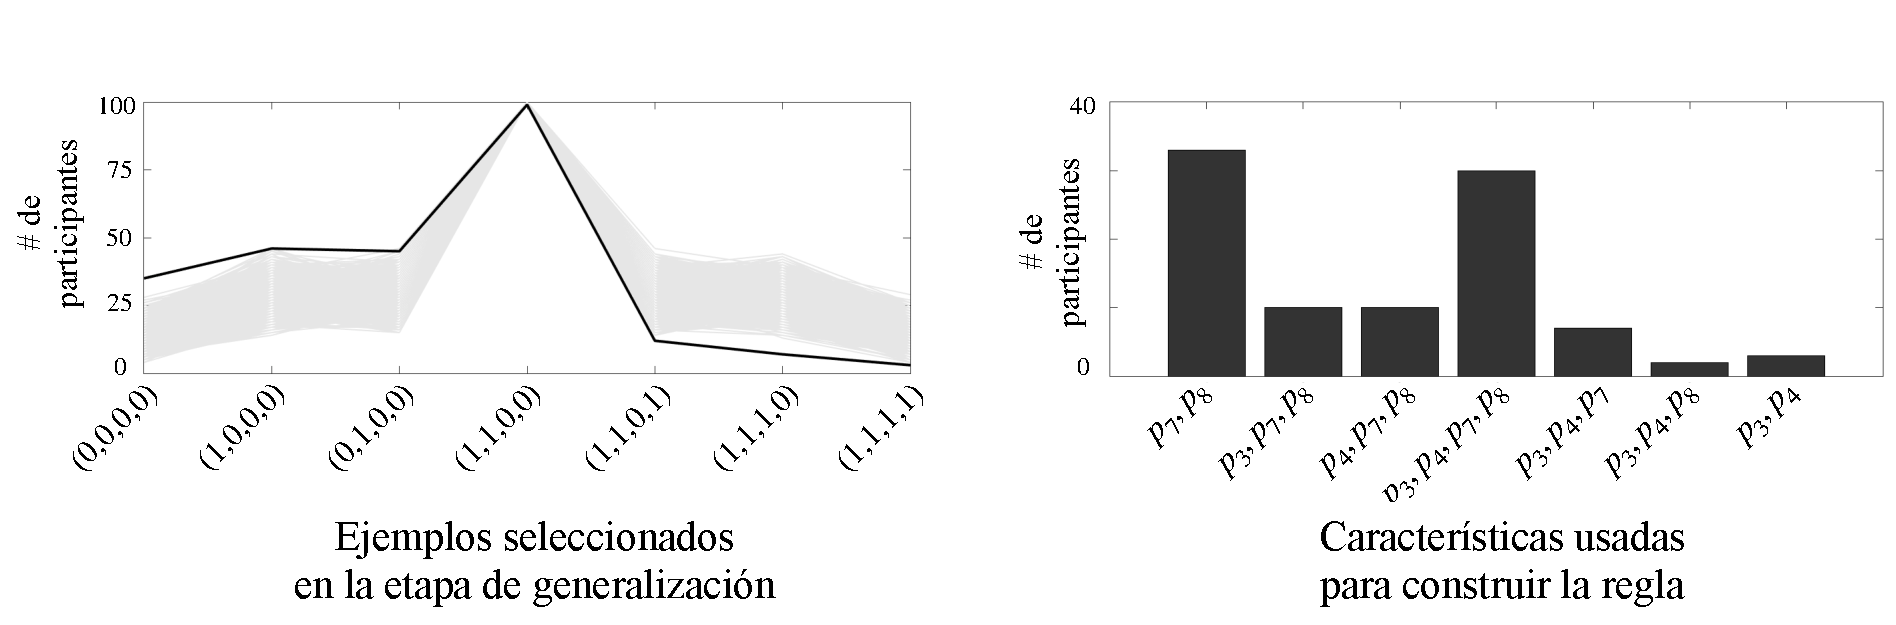
\includegraphics[scale=.4]{papers/images_behavior_research_methods/results_1_sp.pdf}
\end{center}\caption{
% \textbf{(Left)} Number of participants (100 participants total) that, in the generalization stage of Trial 6, selected an element (possibly among others; the numbers add up to more than 100) with the elements written on the x-axis, indicating the values of the features $\{p_3,p_4,p_7,p_8\}$ respectively. As multiple choices were possible, the sum for all choices adds up to a value greater than 100. In grey we show 100,000 simulations in which 100 agents randomly attend to one of the seven subset of features (see text). \textbf{(Right)} From the selected objects in the generalization phase we can infer which features participants used to build the rule for the concept (89 valid participants, see main text).
\textbf{(Izquierda)} Número de participantes (100 participantes en total) que, en la etapa de generalización de la Prueba 6, seleccionaron un elemento (posiblemente entre otros; los números suman más de 100) con los elementos escritos en el eje x, indicando los valores de las características $ \{p_3, p_4, p_7, p_8 \} $ respectivamente. Como eran posibles múltiples opciones, la suma de todas las opciones suma un valor mayor que 100. En gris mostramos 100.000 simulaciones en las que 100 agentes atienden aleatoriamente a uno de los siete subconjuntos de características (ver texto). \textbf{(Derecha)} De los objetos seleccionados en la fase de generalización podemos inferir qué características usaron los participantes para construir la regla para el concepto (89 participantes válidos, ver texto principal).
}
\label{fig:results1}
\end{figure}

 
 \begin{figure}
\begin{center}
	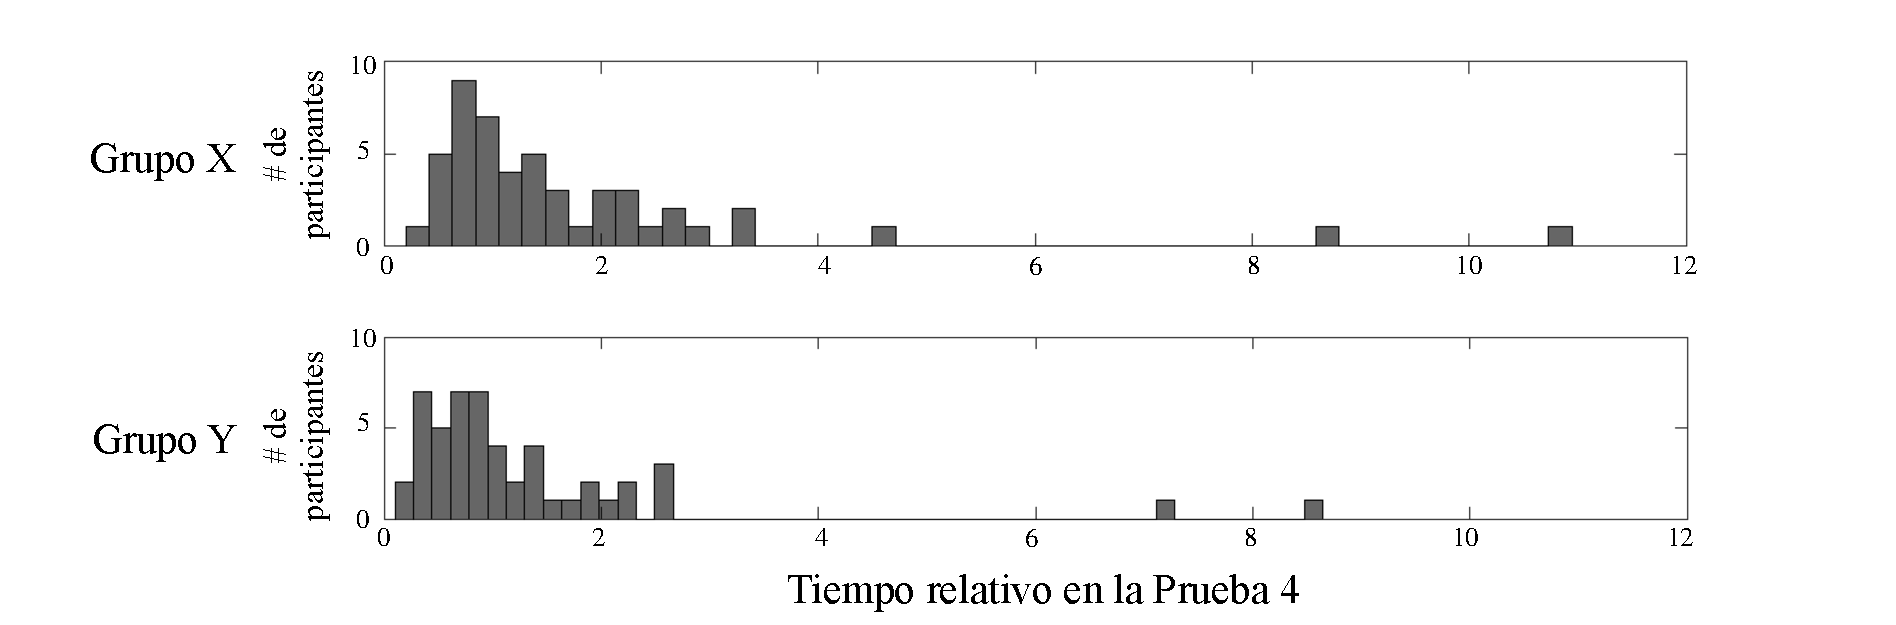
\includegraphics[scale=.5]{papers/images_behavior_research_methods/results_2_sp.pdf}
\end{center}
\caption{
% Relative time spent in Trial 4 by participants from the two groups, normalized by the time spent in Trial 5.
Tiempo relativo empleado en la Prueba 4 por los participantes de los dos grupos, normalizado por el tiempo empleado en la Prueba 5.
}
\label{fig:results2}
\end{figure}



% \subsection{Hypothesis \ref{Hip:FeatureBiasTimeAdvantage}}\label{Results:FeatureBiasTimeAdvantage} 
\subsection{Hipótesis \ref{Hip:FeatureBiasTimeAdvantage}}\label{Results:FeatureBiasTimeAdvantage} 

% This hypothesis regarded the behavioral advantage of the feature stickiness effect, which we tested by comparing learning \emph{times} in Trial 4 for participants of Groups X versus Y (see Figure~\ref{fig:results2}). If the feature stickiness bias represents a behavioral advantage, Group Y should learn concept $C^4_1$ \emph{faster} than Group X. To avoid confounds due to inter-individual differences in absolute learning time, for this analysis we normalize individual learning times with the time spent in Trial 5, which uses different features than the previous concepts and should not be affected by any obvious inter-trial relation with previous concepts\footnote{Indeed, Trial 5 was pre-registered as a `normalizer' trial.}. Thus we compare between the two groups (X and Y) the time spent in Trial 4 divided the time expended in Trial 5. This gives one number for each participant, and we compare the lists of numbers of the two groups using a two-sample t-test.  The differences in the learning times between the groups are not significant if we analyze the data of all participants as shown in Figure~\ref{fig:results2} (two-sample t-test shows $t_{98}=1.26 \ $,  $P=0.2$; Cohen's $d=0.25$), but they are significant if we rule out from this analysis 5 outliers that spent more than 5 times in concept 4 than 5, or in concept 5 than 4 ($t_{98}=2.18 \ $,  $P<0.05$, Cohen's $d=0.42$)\footnote{The ANOVA proposed in the pre-registration also did not reveal significant differences in learning times. For simplicity in the analysis of the outliers, we replaced here the ANOVA for a simple t-test between the normalized learning times of the two groups.}.
Esta hipótesis consideró la ventaja conductual del efecto de adherencia de características, que probamos comparando el tiempo de aprendizaje en la Prueba 4 para los participantes de los Grupos X versus Y (ver Figura~\ref{fig:results2}). Si el sesgo de adherencia de la característica representa una ventaja de comportamiento, el Grupo Y debería aprender el concepto $ C^4_1 $ \emph{más rápido} que el Grupo X. Para evitar confusiones debido a diferencias inter-individuales en el tiempo absoluto de aprendizaje, para este análisis normalizamos el tiempo de aprendizaje individual con el tiempo invertido en la Prueba 5, que utiliza características diferentes a los conceptos anteriores y no debería verse afectado por ninguna relación obvia entre pruebas con conceptos anteriores\footnote{De hecho, la Prueba 5 fue pre-registrada como una prueba `normalizadora'.}. Por lo tanto, comparamos entre los dos grupos (X e Y) el tiempo empleado en la Prueba 4 dividido el tiempo empleado en la Prueba 5. Esto da un número para cada participante, y comparamos las listas de números de los dos grupos usando un t-test de dos muestras. Las diferencias en los tiempos de aprendizaje entre los grupos no son significativas si analizamos los datos de todos los participantes, como se muestra en la Figura~\ref{fig:results2} (el t-test de dos muestras da $ t_{98} = 1.26 \ $, $ P = 0.2 $; $d$ de Cohen $= 0.25 $), pero sí son significativos si descartamos de este análisis 5 valores atípicos que gastaron más de 5 veces en el concepto 4 que en el 5, o en el concepto 5 que en el 4 ($ t_{98} = 2.18 \ $, $ P <0.05 $, $ d$ de Cohen $= 0.42 $)\footnote{El ANOVA propuesto en el pre-registro tampoco reveló diferencias significativas en los tiempos de aprendizaje. Para simplificar el análisis de los valores atípicos, reemplazamos aquí el ANOVA por un t-test simple entre los tiempos de aprendizaje normalizados de los dos grupos.}.



% \subsection{Hypothesis \ref{Hip:StickinessFeatureOperator}} \label{Results:StickinessFeatureOperator} 
\subsection{Hipótesis \ref{Hip:StickinessFeatureOperator}} \label{Results:StickinessFeatureOperator} 

% The idea of this hypothesis is to test if participants prefer sticking to operators or sticking to features form one trial to the next. In this work we did not find conclusive evidence regarding this hypothesis. We suspect that the cause was an experimental setup that underestimated the strength of the bias favoring the $\AND$ operator over the $\OR$ operator. We found that 77 of the 100 participants explained Trial 1 using $\AND$, 11 explained it using $\OR$ and 12 selected elements in the generalization phase with no clear rationale. Of the 77 that used $\AND$, 64 also used $\AND$ in Trial 2, thus changing features but maintaining operator; and 7 of them used $\OR$, changing operator but maintaining features (the other 6 selected elements with no clear rationale). Of the 11 that used $\OR$, 10 used $\AND$ in Trial 2, changing operator but maintaining features; and 1 of them used $\OR$ in the second trial. We realize, however, that a change from using $\OR$ in the first concept to $\AND$ in the second one could not only be due to the effect of feature stickiness, but also simply to the stronger preference for $\AND$. Thus without a precise quantitative knowledge of the prior preference of $\AND$ over $\OR$, we cannot conclude about the effect of operator stickiness vs.\ feature stickiness. A future experiment could probe the existence of operator stickiness by having longer consecutive periods where feature reuse is not a useful bias and where only one logical operator remains useful for explaining a concept, before finally presenting a concept that can be explained via two different rules, each using different operators. Thus we leave for future work the task of studying the interaction between the feature stickiness bias and the precise structure of the logical rules being learnt. 
La idea de esta hipótesis es probar si, de una prueba a la siguiente, los participantes prefieren ceñirse a los operadores o ceñirse a las características. En este trabajo no encontramos evidencia concluyente sobre esta hipótesis. Sospechamos que la causa fue una configuración experimental que subestimó la fuerza del sesgo que favorecía al operador $ \AND $ sobre el operador $ \OR $. Encontramos que 77 de los 100 participantes explicaron la Prueba 1 usando $ \AND $, 11 lo explicaron usando $ \OR $ y 12 de ellos seleccionaron elementos en la fase de generalización sin una justificación clara. De los 77 que usaron $ \AND $, 64 también usaron $ \AND $ en la Prueba 2, cambiando así las características pero manteniendo el operador; y 7 de ellos usaron $ \OR $, cambiando de operador pero manteniendo las características (los otros 6 participantes seleccionaron elementos sin una justificación clara). De los 11 que usaron $ \OR $, 10 usaron $ \AND $ en la Prueba 2, cambiando de operador pero manteniendo las características; y 1 de ellos usó $ \OR $ en la segunda prueba. Sin embargo, nos damos cuenta de que un cambio de usar $ \OR $ en el primer concepto a $ \AND $ en el segundo podría deberse no solo al efecto de la adherencia de las características, sino también simplemente a la preferencia más fuerte por $ \AND$. Por lo tanto, sin un conocimiento cuantitativo preciso de la preferencia previa de $ \AND $ sobre $ \OR $, no podemos concluir nada sobre el efecto de la adherencia del operador frente a la adherencia de la característica. Un experimento futuro podría probar la existencia de adherencia de operador al tener períodos consecutivos más largos donde la reutilización de características no es un sesgo útil y donde solo un operador lógico sigue siendo útil para explicar un concepto, antes de presentar finalmente un concepto que se puede explicar a través de dos reglas diferentes, cada uno usando diferentes operadores. De este modo, dejamos para el trabajo futuro la tarea de estudiar la interacción entre el sesgo de adherencia de características y la estructura precisa de las reglas lógicas que se están aprendiendo.\santi{aca hay algo que podes mandar a una seccion final en la tesis sobre trabajo futuro}


% \subsection{MDL bias} \label{Resultados:MDLbias} 
\subsection{El sesgo de MDL} \label{Resultados:MDLbias} 


% The MDL-bias hypothesis posits that concept-learning difficulty increases with its MDL~\cite{feldman2000minimization}. In addition to their other roles, Trials 3 (group X and Y), 4, and 5 served to test this hypothesis in the new framework of multiple consistent explanations. In these trials, there were two possible explanations that were consistent with the shown data, one of much higher MDL than the other (15 vs.\ 3). For example, in the Group X of Trial~3, the short explanation was $p_1 \land p_2$, while the longer one was $((p_3 \lor (p_4 \lor p_5))\land(\lnot p_3 \lor ((p_4 \lor \lnot p_5)\land (p_5 \lor \lnot p_4))))$; the longer rule in other trials was always a substitution of features applied to this one (in order to keep the features disjoint between the two explanations). For these 3 trials, the responses of the $100$ participants add to a total of $300$ responses. From this total, $18$ responses in the generalization phase did not choose objects consistent with any of the two explanations; $2$ responses were consistent with the MDL~15 rule; and $280$ responses were consistent with the MDL~3 rule. While this was expected by the experimental design (since we included a MDL~15 rule in those trials where we wanted to bias the participants into finding the other rule), we conclude that the MDL-bias hypothesis holds in this framework of multiple consistent explanations. Future work could explore in greater detail the relative difficulty of rules with slightly different MDL in this framework.
La hipótesis del sesgo de MDL postula que la dificultad de aprendizaje de conceptos aumenta con su MDL~\cite{feldman2000minimization}. Además de sus otros roles, las Pruebas 3 (grupo X e Y), 4 y 5 sirvieron para probar esta hipótesis en el nuevo marco de múltiples explicaciones consistentes. En estas pruebas, hubo dos posibles explicaciones que eran consistentes con los datos mostrados, una de MDL mucho más alta que la otra (15 vs.\ 3). Por ejemplo, en el Grupo X de la Prueba~3, la explicación corta fue $ p_1 \land p_2 $, mientras que la más larga fue $ ((p_3 \lor (p_4 \lor p_5)) \land (\lnot p_3 \lor ( (p_4 \lor \lnot p_5) \land (p_5 \lor \lnot p_4)))) $; la regla más larga en otras pruebas fue siempre una sustitución de características aplicadas a este (para mantener las características disjuntas entre las dos explicaciones). Para estas 3 pruebas, las respuestas de los $ 100 $ participantes suman un total de $ 300 $ respuestas. De este total, las respuestas de $ 18 $ en la fase de generalización no eligieron objetos consistentes con ninguna de las dos explicaciones; $ 2 $ respuestas fueron consistentes con la regla de MDL~15; y $ 280 $ respuestas fueron consistentes con la regla de MDL~3. Si bien esto era lo esperable por el diseño experimental (dado que incluimos una regla de MDL~15 en aquellas pruebas en las que queríamos sesgar a los participantes para que encontraran la otra regla), concluimos que la hipótesis del sesgo de MDL se mantiene en este marco de múltiples explicaciones consistentes. Un trabajo futuro podría explorar con mayor detalle la dificultad relativa de las reglas con MDL ligeramente diferente en este marco.\santi{idem}



% \section{Discussion}\label{sec:Discussion}
\section{Discusión}\label{sec:Discussion}


% In this work,  we  design  an experimental framework in which participants observe an incomplete set of examples, which are consistent with two alternative minimal descriptions depending on which features are observed.  We  illustrate  several advantages of our method compared to separately presenting sets of examples consistent with only one minimal description at a time. First, we  show  that when a set of examples is consistent with a disjunction \textit{and also} with a conjunction, participants are more likely to find the conjunction, in accordance with well-known previous results that show that the conjunction is learnt faster than the disjunction when presented separately~\cite{bourne1970knowing}. Then, we  show  that when rules of significantly different MDL are consistent with the observations, almost all participants discover the simpler rules, consistent with previous result showing that, when rules of different MDL are tested separately, learning times are proportional to MDLs~\cite{feldman2000minimization}. Finally, we  show  that when the logical structure of the minimal rules is independent of the selected features, participants are more likely to reuse the same features used to describe previous concepts,  and preliminary results suggest that reusing features  allows them to learn concepts faster than a control group that is not reusing features. To our knowledge this effect has not been previously characterized in the concept-learning literature, adding to the library of effects illustrating how human attention is biased towards features that are useful to describe the concepts (see~\cite{blair2009extremely,kruschke2000blocking,kruschke2005eye,hoffman2010costs}, among others).
En este trabajo, diseñamos un marco experimental en el que los participantes observan un conjunto incompleto de ejemplos, que son consistentes con dos descripciones mínimas alternativas según las características que se observen. Ilustramos varias ventajas de nuestro método en comparación con la presentación por separado de conjuntos de ejemplos consistentes con solo una descripción mínima a la vez. Primero, mostramos que cuando un conjunto de ejemplos es consistente con una disyunción \textit{y también} con una conjunción, es más probable que los participantes encuentren la conjunción, de acuerdo con resultados previos bien conocidos que muestran que la conjunción se aprende más rápido. que la disyunción cuando se presentan por separado~\cite{bourne1970knowing}. Luego, mostramos que cuando las reglas con MDL significativamente diferentes son consistentes con las observaciones, casi todos los participantes descubren las reglas más simples, consistentes con el resultado anterior que muestra que, cuando las reglas con MDL diferentes se testean por separado, los tiempos de aprendizaje son proporcionales a las MDLs~\cite{feldman2000minimization}. Finalmente, mostramos que cuando la estructura lógica de las reglas mínimas es independiente de las características seleccionadas, es más probable que los participantes reutilicen las mismas características usadas para describir conceptos anteriores, y los resultados preliminares sugieren que la reutilización de características les permite aprender conceptos más rápido que un grupo de control que no está reutilizando características. Hasta donde sabemos, este efecto no se ha caracterizado previamente en la literatura sobre el aprendizaje de conceptos, lo que se suma a la biblioteca de efectos que ilustran cómo la atención humana está sesgada hacia características que son útiles para describir los conceptos (ver~\cite{blair2009extremely, kruschke2000blocking, kruschke2005eye, hoffman2010costs}, entre otros).


% Eye-tracking studies in categorization tasks have revealed that feature attention rapidly changes between trials depending on which features are relevant for classification in each trial~\cite{blair2009extremely}, as well as depending on prior knowledge about feature relevance~\cite{kim2011prior}. In~\cite{kruschke2005eye} it is found that eye movements confirmed that attention was learned in the basic learned inhibition paradigm, and in~\cite{hoffman2010costs} it is also found that eye movements revealed how an attention profile learned during a first phase of learning affected a second phase.  Our experimental setup allows us to test an arguably simpler complementary hypothesis: everything else being equal, participants are biased to use the same features used in the past.  Importantly, we were only able to test this hypothesis thanks to our framework, which allows us to present a set of examples consistent with two rules of exactly the same logical structure, but using different sets of features. Then, without using eye-tracking, we can recover which rule the participants learned, and thus which set of features they attended to. Since the two sets of features explain the examples using exactly the same logical structure, preferentially explaining the concept using one set of features over the other can only be due to a preference over the features themselves, and not a preference over alternative logical structures. 
Los estudios de seguimiento ocular ({\em eye tracking}) en las tareas de categorización han revelado que la atención a las características cambia rápidamente entre pruebas dependiendo de qué características son relevantes para la clasificación en cada ensayo~\cite{blair2009extremely}, así como según el conocimiento previo sobre la relevancia de las características~\cite{kim2011prior}. En \cite {kruschke2005eye} se encuentra que los movimientos oculares confirmaron que la atención se aprendió en el paradigma básico de inhibición aprendida, y en~\cite{hoffman2010costs} también se encontró que los movimientos oculares revelaron cómo un perfil de atención aprendido durante una primera fase de aprendizaje afectó una segunda fase. Nuestra configuración experimental nos permite probar una hipótesis complementaria posiblemente más simple: si todo lo demás permanece igual, los participantes están predispuestos a usar las mismas características que se usaron en el pasado. Es importante destacar que solo pudimos probar esta hipótesis gracias a nuestro marco, que nos permite presentar un conjunto de ejemplos consistentes con dos reglas de exactamente la misma estructura lógica, pero usando diferentes conjuntos de características. Luego, sin usar el seguimiento ocular, podemos recuperar qué regla aprendieron los participantes y, por lo tanto, a qué conjunto de características prestaron atención. Dado que los dos conjuntos de características explican los ejemplos usando exactamente la misma estructura lógica, explicar preferentemente el concepto usando un conjunto de características sobre el otro solo puede deberse a una preferencia sobre las características en sí mismas, y no una preferencia sobre estructuras lógicas alternativas.



% Although some of the hypothesis that we test are aligned with the well-known Einstellung effect which states that adopted solutions may hinder simpler ones when aiming at tackling novel problems, our experimental setting is different to the classical water jar test (the most commonly cited example of an Einstellung effect, where participants need to discover how to measure a certain amount of water using three jars with different and fixed capacity) ~\cite{luchins1942mechanization} in two senses. First, we do not drive the experiment to control and supervise the aspects that participants have to pay attention to. On the contrary, our focus is on the {\em choice} of the features that show to be useful for learning a concept with more than one rational explanation. Second, our experimental framework is consistent with the Language of Thought (LoT) hypothesis~\cite{fodor1975language}, which states that the human capacity to describe concepts —and, more generally, of all elements of thought— builds on the use of a symbolic and combinatorial mental language and it is specifically conceived to handle expressions in propositional Logic (but expansible to other formal languages), which is the ground where the rational explanations can be formalized. Such approach enables us to treat the notion of {\em feature} in a very precise way. 
Aunque algunas de las hipótesis que probamos están alineadas con el conocido efecto Einstellung, que establece que las soluciones adoptadas pueden obstaculizar las más simples al tratar de abordar problemas nuevos, nuestro entorno experimental es diferente a la prueba clásica de la jarra de agua (el ejemplo más comúnmente citado de un efecto Einstellung, donde los participantes necesitan descubrir cómo medir una cierta cantidad de agua usando tres jarras con capacidad diferente y fija)~\cite{luchins1942mechanization} en dos direcciones. Primero, no condujimos el experimento para controlar y supervisar los aspectos a los que los participantes deben prestar atención. Por el contrario, nuestro enfoque está en la {\em elección} de las características que demuestran ser útiles para aprender un concepto con más de una explicación racional. En segundo lugar, nuestro marco experimental es coherente con la hipótesis del lenguaje del pensamiento (LoT)~\cite{fodor1975language}, que establece que la capacidad humana para describir conceptos —-y, más generalmente, de todos los elementos del pensamiento-— se basa en el uso de un lenguaje mental simbólico y combinatorio, y está específicamente concebido para manejar expresiones en lógica proposicional (pero expansible a otros lenguajes formales), que es el terreno donde se pueden formalizar las explicaciones racionales. Este enfoque nos permite tratar la noción de {\em característica} de una manera muy precisa.\santi{esta parte de LoT seguramente se vaya porque vas a haber hablado mucho ya sobre esto en la intro.}


% We note that other frameworks besides LoT can be used for our experiment. For example, consider similarity-based classification rules~\cite{juslin2003cue,juslin2003exemplar}, where each feature is multiplied by a weight and the classification rule is a function of the sum of the weighted features, usually a linear function with a soft decision boundary~\cite{juslin2003exemplar}. In this framework, the generalization phase would determine which of two possible decision boundaries was used by the participants (both consistent with the elements observed in the learning phase); and the feature-stickiness effect would be explained by the inertia of the weights' values from one concept to the next. However, two obstacles in this framework makes us prefer the LoT framework for Boolean concept-learning tasks. First, although a linear classification rule can readily learn the conjunctions and disjunctions in our experiment, more complex classification rules would require nonlinear functions of the features (e.g.\ the exclusive-or (XOR)). For nonlinear boundaries, the values of the weights that accompany the features could be hard to interpret, since it might no longer be true that a higher weight means higher feature importance. In contrast, in the LoT framework complex classification rules are compositionally built to accommodate concepts of any complexity, and feature importance can always be modeled as the probability of including a feature in a formula, independently of its complexity. Second, unlike similarity-based rules, the LoT framework naturally explains how humans can built verbal explanations for the learned concepts. Indeed, almost all participants gave informal explanations of conjunctions and disjunctions in propositional logic after learning each concept (see the shared data online for the list of verbal explanations). 
Observamos que se pueden utilizar otros marcos además de LoT para nuestro experimento. Por ejemplo, consideremos las reglas de clasificación basadas en similitudes~\cite{juslin2003cue, juslin2003exemplar}, donde cada característica se multiplica por un peso y la regla de clasificación es una función de la suma de las características ponderadas, generalmente una función lineal con un límite de decisión suave~\cite{juslin2003exemplar}. En este marco, la fase de generalización determinaría cuál de los dos posibles límites de decisión fue utilizado por los participantes (ambos consistentes con los elementos observados en la fase de aprendizaje); y el efecto de adherencia de características se explicaría por la inercia de los valores de los pesos de un concepto al siguiente. Sin embargo, dos obstáculos en este marco nos hacen preferir el marco de LoT para las tareas de aprendizaje de conceptos booleanos. Primero, aunque una regla de clasificación lineal puede aprender fácilmente las conjunciones y disyunciones en nuestro experimento, las reglas de clasificación más complejas requerirían funciones no lineales de las características (por ejemplo, el o-exclusivo (XOR)). Para los límites no lineales, los valores de las ponderaciones que acompañan a las características pueden ser difíciles de interpretar, ya que puede que ya no sea cierto que una ponderación más alta signifique una mayor importancia de las características. En contraste, en el marco de trabajo de LoT, las reglas de clasificación complejas se construyen de manera compositiva para acomodar conceptos de cualquier complejidad, y la importancia de las características siempre se puede modelar como la probabilidad de incluir una característica en una fórmula, independientemente de su complejidad. En segundo lugar, a diferencia de las reglas basadas en similitudes, el marco de LoT explica naturalmente cómo los humanos pueden construir explicaciones verbales para los conceptos aprendidos. De hecho, casi todos los participantes dieron explicaciones informales de conjunciones y disyunciones en la lógica proposicional después de aprender cada concepto (consultar los datos compartidos en línea para ver la lista de explicaciones verbales).


% Another well-studied phenomenon related to our work is Kamin’s cue {\em blocking}, where the learning of a given stimulus B is {\em blocked} by the mere fact that it was preceded by a set of stimuli A that already pairs with the outcome. This shows that the subject learned that stimulus B was not useful, and hence disregards their attention to it in the upcoming events~\cite{wagner1970stimulus,mackintosh1975theory,rescorlaw72}. Studied in humans in~\cite{chapman1990cue, arcediano1997blocking, kruschke2000blocking} among others, our work differs from these approaches in that we never introduce a stage were a feature A is intentionally exposed in absence to B, in order to guide the attention of the participant.
Otro fenómeno bien estudiado relacionado con nuestro trabajo es el {\em blocking} de Kamin, donde el aprendizaje de un estímulo B dado está {\em bloqueado} por el mero hecho de que fue precedido por un conjunto de estímulos A que ya se empareja con el resultado. Esto muestra que el sujeto aprendió que el estímulo B no era útil y, por lo tanto, ignora su atención en los eventos siguientes~\cite{wagner1970stimulus, mackintosh1975theory, rescorlaw72}. Estudiado en humanos en~\cite{chapman1990cue, arcediano1997blocking, kruschke2000blocking} entre otros, nuestro trabajo se diferencia de estos enfoques en que nunca introducimos una etapa donde una característica A se expone intencionalmente en ausencia de B, con el fin de orientar la atención del participante.


% We conjecture that most first-order determinants of subjective concept difficulty will also hold in a relative manner in our dual-concept setup, such as the MDL bias (for less extreme cases than evaluated in this work)~\cite{feldman2003simplicity} and the transfer learning hierarchical structure bias~\cite{tano2020towards}. Importantly, our experimental setup also allows to directly test second-order subjective difficulty effects (e.g.\ concept A is learnt faster if presented jointly with concept B than with concept C), as well as second-order transfer learning effects (e.g.\  participants learn more rapidly concept C if they have first observed concept A coupled with B$_1$, compared to A coupled with B$_2$). We believe that a systematic study of concept-learning difficulty with two (or more) concepts presented at the same time in each trial may open a new window into the dynamics of human concept-learning mechanisms. For example, consider the study in~\cite{piantadosi2016logical}, where participants gradually learn one concept while simultaneously selecting elements currently believed to belong to that concept. Here, the authors fit a Bayesian language model to participants' choices in order to illustrate how the posterior probability of the different rules in the grammar varied across time, to approximate the order in which different rules are learned. In contrast, using our experimental setting we can directly estimate, in a model-free manner, the probability that each rule is learnt faster than another. One simply needs to jointly present (in an incomplete and mutually compatible way) a set of examples consistent with those two minimal rules, and then measure the fraction of participants that discover each rule.
Conjeturamos que la mayoría de los determinantes de primer orden de la dificultad del concepto subjetivo también se mantendrán de manera relativa en nuestra configuración de concepto dual, como el sesgo de MDL (para casos menos extremos que los evaluados en este trabajo)\cite{feldman2003simplicity} y el sesgo de la estructura jerárquica del aprendizaje por transferencia~\cite{tano2020towards}. Es importante destacar que nuestra configuración experimental también permite probar directamente los efectos de dificultad subjetiva de segundo orden (por ejemplo, el concepto A se aprende más rápido si se presenta junto con el concepto B que con el concepto C), así como los efectos de aprendizaje de transferencia de segundo orden (por ejemplo, los participantes aprenden más rápidamente el concepto C si primero han observado el concepto A junto con B$_1 $, en comparación con A junto con B $_2$). Creemos que un estudio sistemático de la dificultad de aprendizaje de conceptos con dos (o más) conceptos presentados al mismo tiempo en cada prueba puede abrir una nueva ventana a la dinámica de los mecanismos humanos de aprendizaje de conceptos. Por ejemplo, consideremos el estudio en~\cite{piantadosi2016logical}, donde los participantes aprenden gradualmente un concepto mientras simultáneamente seleccionan elementos que actualmente se creen que pertenecen a ese concepto. Aquí, los autores ajustan un modelo bayesiano de lenguaje a las elecciones de los participantes para ilustrar cómo la probabilidad posterior de las diferentes reglas en la gramática varió a lo largo del tiempo, para aproximar el orden en el que se aprenden las diferentes reglas. Por el contrario, utilizando nuestro entorno experimental podemos estimar directamente, sin modelos, la probabilidad de que cada regla se aprenda más rápido que otra. Uno simplemente necesita presentar conjuntamente (de una manera incompleta y mutuamente compatible) un conjunto de ejemplos consistentes con esas dos reglas mínimas, y luego medir la fracción de participantes que descubre cada regla.


% Usually, concept-learning biases have been studied in an isolated manner: the participant observes examples indicated as inside or outside a \textit{single} concept, and the experimenter evaluates its subjective difficulty for the participant. Although different methods have been used to present the concept to the participant (e.g.\ all elements at the same time~\cite{tano2020towards,kemp2012exploring} or small sets of elements presented in series~\cite{piantadosi2016logical}), to the best of our knowledge all previous category-learning studies have attempted to evaluate a single concept at a time. Here, we present a controlled logical setting to evaluate the relative difficulty of two concepts presented at the same time and under the same experimental conditions, and the framework could be generalized to more concepts straightforwardly. 
Por lo general, los sesgos de aprendizaje de conceptos se han estudiado de manera aislada: el participante observa ejemplos indicados como dentro o fuera de un concepto \textit{único}, y el experimentador evalúa su dificultad subjetiva para el participante. Aunque se han utilizado diferentes métodos para presentar el concepto al participante (por ejemplo, todos los elementos al mismo tiempo~\cite{tano2020towards, kemp2012exploring} o pequeños conjuntos de elementos presentados en serie~\cite{piantadosi2016logical}), por lo que sabemos todos los estudios previos de aprendizaje de categorías han intentado evaluar un solo concepto a la vez. Aquí, presentamos un escenario lógico controlado para evaluar la dificultad relativa de dos conceptos presentados al mismo tiempo y bajo las mismas condiciones experimentales, y, de forma directa, nuestro marco podría generalizarse a más.



% \paragraph{Open Practices Statement.} 
\paragraph{Declaración de prácticas abiertas.} 
% This study's methodology, data collection procedures, sample size, exclusion criteria, and hypotheses were preregistered on the Open Science Framework (OSF) in advance of the data collection and analysis, in order to ensure transparency, reproducibility, and rigour. The preregistration of this study can be found at \url{https://osf.io/mgex3}. The actual experiment as presented to the participants, together with all the experimental data analyzed, is available online at \url{https://osf.io/gtuwp/}.
La metodología de este estudio, los procedimientos de recopilación de datos, el tamaño de la muestra, los criterios de exclusión y las hipótesis se registraron previamente en el Open Science Framework (OSF) antes de la recopilación y el análisis de datos, con el fin de garantizar la transparencia, la reproducibilidad y el rigor. El pre-registro de este estudio se puede encontrar en \url{https://osf.io/mgex3}. El experimento real presentado a los participantes, junto con todos los datos experimentales analizados, está disponible en línea en \url{https://osf.io/gtuwp/}.

%\bibliographystyle{apalike} 
%\bibliography{biblioCategorization}



